\documentclass[10pt]{article}
\usepackage{geometry}
\geometry{a4paper}
\pagestyle{myheadings}
\usepackage{tikz}
\usepackage{pgfplots}
\usepackage{fancyhdr} % Required for custom headers
\usepackage{lastpage} % Required to determine the last page for the footer
\usepackage{extramarks} % Required for headers and footers
\usepackage{graphicx} % Required to insert images
\usepackage{listings} % Required for insertion of code
\usepackage{courier} % Required for the courier font
\usepackage{caption}
\usepackage{subcaption}
\usepackage{amsmath}
\usepackage{amsfonts}
\usepackage{amssymb}
\usepackage{epstopdf}
\usepackage{placeins}
\usepackage{fancyvrb} 
\usepackage[numbered]{bookmark}
\usepackage{pgfplots}
\usepackage{ifthen}
\usepackage{enumitem}
\usepackage{setspace}
\usepackage{placeins} % for FloatBarrier
\usepackage[makeroom]{cancel}
\usepackage[absolute,overlay]{textpos}
\usetikzlibrary{calc, angles,quotes}
\usetikzlibrary{pgfplots.fillbetween, backgrounds}
\usetikzlibrary{positioning}
\usetikzlibrary{arrows}
\usetikzlibrary{pgfplots.groupplots}
\usetikzlibrary{arrows.meta}
\usetikzlibrary{plotmarks}
\usetikzlibrary{decorations.markings}

\usepgfplotslibrary{groupplots}
\pgfplotsset{compat=newest} 

\DeclareGraphicsExtensions{.pdf,.png,.jpg}
\graphicspath{{../figs/}}

\definecolor{blue2}{RGB}{51, 105, 232}  
\definecolor{red2}{RGB}{213, 15, 37}  
\definecolor{green2}{RGB}{0, 153, 37}  

\definecolor{matlabcomment}{RGB}{34,139,34}

\pgfmathdeclarefunction{gauss}{1}{%
	\pgfmathparse{1/(sqrt(2*pi))*exp(-((#1)^2)/2)}%
}

\pgfmathdeclarefunction{laplacian}{2}{%
	\pgfmathparse{1/(#2*2)*exp(-(abs(x-#1))/(#2))}%
}

\pgfmathdeclarefunction{pretty_func}{1}{%
	\pgfmathparse{cos(deg(#1/2)) - sin(deg(#1)) + cos(deg(#1/2)-45) - sin(deg(#1/4)-154)}%
}

\pgfplotsset{
	dirac/.style={
		mark=triangle*,
		mark options={scale=2},
		ycomb,
		scatter,
		visualization depends on={y/abs(y)-1 \as \sign},
		scatter/@pre marker code/.code={\scope[rotate=90*\sign,yshift=-2pt]}
	}
}

\def\thickness{very thick}

\tikzset{
amark/.style 2 args={
	decoration={             
		markings, 
		mark=at position {0.5} with { 
			\arrow{stealth},
			\node[#2] {#1};
		}
	}, \thickness,
	postaction={decorate}
},
earlymark/.style 2 args={
	decoration={             
		markings, 
		mark=at position {0.25} with { 
			\arrow{stealth},
			\node[#2] {#1};
		}
	}, \thickness,
	postaction={decorate}
},
latemark/.style 2 args={
	decoration={             
		markings, 
		mark=at position {0.8} with { 
			\arrow{stealth},
			\node[#2] {#1};
		}
	}, \thickness,
	postaction={decorate}
},
zpath/.style={
	decoration={             
		markings, 
		mark=at position {0.5} with { 
			\arrow{stealth},
			\node[#1] {$z^{-1}$};
		}
	}, \thickness,
	postaction={decorate}
},
terminal/.style 2 args={draw,circle,inner sep=2pt,label={#1:#2}},
}


\tikzset{
	invisible/.style={opacity=0},
	visible on/.style={alt={#1{}{invisible}}},
	alt/.code args={<#1>#2#3}{%
		\alt<#1>{\pgfkeysalso{#2}}{\pgfkeysalso{#3}} % \pgfkeysalso doesn't change the path
	},
}

\newcommand\PlotSampledSpectrum[4]{%
	\def\fs{#2}%
	\def\fmax{#3}%
	\def\ros{#4}%
	\input{#1}%
}

\pgfmathdeclarefunction{invgauss}{2}{%
	\pgfmathparse{sqrt(-2*ln(#1))*cos(deg(2*pi*#2))}%
}

\tikzset{
	declare function={
		sinc(\x) = (and(\x!=0, 1) * (sin(deg(pi*\x))/(pi*\x)) +
		(and(\x==0, 1) * 1);
	}
}

\DeclareMathOperator{\E}{\mathbb{E}} % expectation

\newcommand\SimpleSys[4]{%
	\def\xin{#2}%
	\def\Hz{#3}%
	\def\yout{#4}
	\input{#1}%
}

%%%%%%%%%%%%% SOLUTIONS %%%%%%%%%%%%%%%%%
\def\SOLUTIONS{0} % change to 1 to produce solutions
\def\SolutionsColor{red2}
%%%%%%%%%%%%%%%%%%%%%%%%%%%%%%%%%%%%%%%%%

% Header
\if\SOLUTIONS1
	\markboth{\em \color{\SolutionsColor} \textbf{EE264: Final exam solutions}}{\em \color{\SolutionsColor} \textbf{EE264: Final exam solutions}}
    \title{EE 264 Final exam solutions}
\else
	\markboth{\em EE264: Final Exam, Summer 2018}{\em EE264: Final Exam, Summer 2018}
    \title{EE 264 Final}
\fi

% Document
\begin{document}
\doublespacing
\begin{center}
\textbf{\Large Stanford University}

\textbf{\Large Department of Electrical Engineering}

\Large EE 264: Digital Signal Processing 

\Large Final Exam

\Large Summer, 2017
\end{center}
\vspace{-0.5cm}
\rule{\textwidth}{1pt}

\noindent\textbf{Name:} \rule{0.4\textwidth}{0.5pt} \qquad  \textbf{Date and time:} \rule{0.3\textwidth}{0.5pt}

\noindent\textbf{SUNet ID:} \rule{0.3\textwidth}{0.5pt}\qquad 
\textbf{SCPD Student?} yes no

\mbox{}\\
\textbf{Instructions:}
\singlespacing
\begin{enumerate}
\item This is a 24h-take home exam. 
\item Carefully read over and understand the exam problems before you start.
\item The exam is open book and open notes. You may use all available references.
\item Be clear, organized, and concise in your answers.
\item Please submit your solutions in a single .pdf file on Canvas. Your submission \underline{must} include this cover page signed. 
\item Do \underline{not} communicate with others about the exam even after you have taken it, as some students will take the exam at a different time.
\item If you have questions during the exam, please contact the teaching staff \{jkperin, trumu\}@stanford.edu. However, we will not provided additional hints or check your answers.
\end{enumerate}

\noindent\textbf{The Stanford University Honor Code:}
\begin{quote}
I attest that I have not given or received aid in this examination, and that I have done my share and taken an active part in seeing to it that others as well as myself uphold the spirit and letter of the Honor Code.
\end{quote}
\vspace{1mm}

\begin{center}\textbf{Signature:} \rule{0.7\textwidth}{0.5pt}\end{center}

\doublespacing
\vspace{0.1cm}
\begin{center}
\begin{tabular}{ccc}
\textbf{Problem} & \textbf{Points} & \textbf{Score} \\
1 & 55 & \\
2 & 45 & \\
\end{tabular}
\end{center}
\singlespacing
\pagebreak


\section*{Problem 1: Hearing aid (60 points)}

Figure~\ref{fig:hearing_aid_diagram} shows the block diagram of a hearing aid device. The signal recorded by the microphone is low-pass filtered by the anti-aliasing filter $H_{aa}(j\Omega)$, and then converted to digital domain by the ADC. A digital filter $H(z)$ corrects for the patient's hearing loss by boosting the signal at particular frequencies or band of frequencies. Once the signal has been filtered, it is converted back to the analog domain using a DAC, which will then drive a speaker that is placed inside the patient's hearing canal. 

\FloatBarrier
\begin{figure}[h!]
	\centering
	\resizebox{\textwidth}{!}{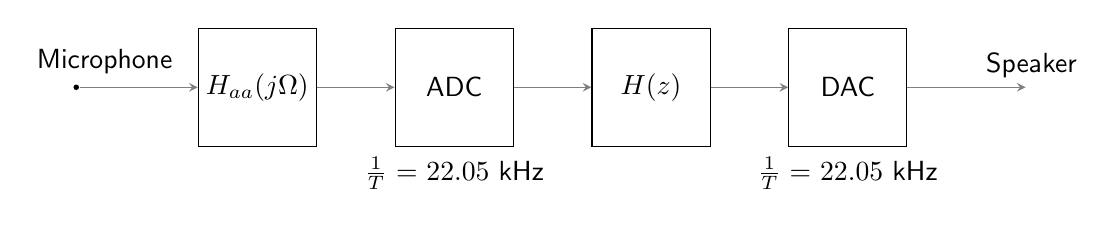
\begin{tikzpicture}[->, >=stealth, shorten >= 0pt, draw=black!50, node distance=2.5cm, font=\sffamily]
    \tikzstyle{node}=[circle,fill=black,minimum size=2pt,inner sep=0pt]
    \tikzstyle{block}=[draw=black,rectangle,fill=none,minimum size=1.5cm, inner sep=0pt]

	\node[node] (xc) {};
	\node[block, right=1.5cm of xc] (Haa) {$H_{aa}(j\Omega)$};
    \node[block, right of=Haa] (ADC) {ADC};
    \node[block, right of=ADC] (DSP) {$H(z)$};
    \node[block, right of=DSP] (DAC) {DAC};
	\coordinate[right=1.5cm of DAC] (yc) {};
		
    \path (xc) edge (Haa);
    \path (Haa) edge (ADC);
    \path (ADC) edge (DSP);
    \path (DSP) edge (DAC);
    \path (DAC) edge (yc);
    
    \node[above = 0mm of xc, text width = 1cm, align=center] {Microphone};
    \node[above = 0mm of yc, text width = 1cm, align=center] {Speaker};
    \node[below, align=center, text width=2.5cm] at ($(ADC.south)$) {$\frac{1}{T} = 22.05$ kHz};
    \node[below, align=center, text width=2.5cm] at ($(DAC.south)$) {$\frac{1}{T} = 22.05$ kHz};
\end{tikzpicture}}
	\caption{Block diagram of a digital hearing aid device.}
	\label{fig:hearing_aid_diagram}
\end{figure}
\FloatBarrier

\FloatBarrier
\begin{figure}[h!]
	\centering
	\resizebox{0.7\textwidth}{!}{\begin{tikzpicture}
\begin{axis}[
%axis lines*=middle,
enlargelimits = false, clip=true,
scale only axis,
axis line style={->,>=stealth, shorten >= 0pt},
xlabel={Frequency (Hz)},
ylabel={Hearing loss (dB)},
every outer x axis line/.append style={white!15!black},
every x tick label/.append style={font=\color{white!15!black}},
xmin=0, xmax=10,
ymin=-60, ymax=10,
xtick={0.5, 1, 2, 3, 4, 5, 6, 7, 8, 9, 10},
ymajorgrids,
xmajorgrids,
every outer y axis line/.append style={white!15!black},
every y tick label/.append style={font=\color{white!15!black}},
legend style={draw=white!15!black,fill=white,legend cell align=left, at={(axis cs: 1.05, -5)}}]

\addplot [smooth, color=black, mark=*, mark size = 3pt, mark options={fill=white}, solid, line width=2pt] table[x index=0,y index=1] {figs/adiogram.dat}; 

\end{axis}
\end{tikzpicture}


% each nth point={100}
% restrict x to domain=1:4}
	\caption{Audiogram of patient.}
	\label{fig:audiogram}
\end{figure}
\FloatBarrier

Figure~\ref{fig:audiogram} shows the \textit{audiogram} of a given patient. This plot shows the patient's hearing loss at particular frequencies. For instance, a hearing loss of 0 dB means that no correction needs to be done at that frequency. However, this patient has a hearing loss of 50 dB at 10 kHz. Hence, the system must provide a gain of nearly 50 dB at 10 kHz. The data from this plot is available in the file \texttt{hearing\_aid.m}. 

For the following questions assume that the sampling rate of the ADC is $1/T = 22.05$ kHz, and the same sampling rate is used for reconstruction.
\begin{enumerate}[label=(\alph*)]
	\item (5 points) Plot the desired filter specification $|H_d(e^{j\omega})|$ that would compensate for the patient's hearing loss. The $x$-axis of your plot should be the normalized frequency $\omega$ or $\omega/\pi$, while the $y$-axis should be the magnitude $20\log_{10}(|H_d(e^{j\omega})|)$ in dB.
	
	\if\SOLUTIONS1
	{\color{\SolutionsColor} The filter specification is simply the inverse of the patient's hearing loss.
		
		\FloatBarrier
		\begin{figure}[h!]
			\centering
			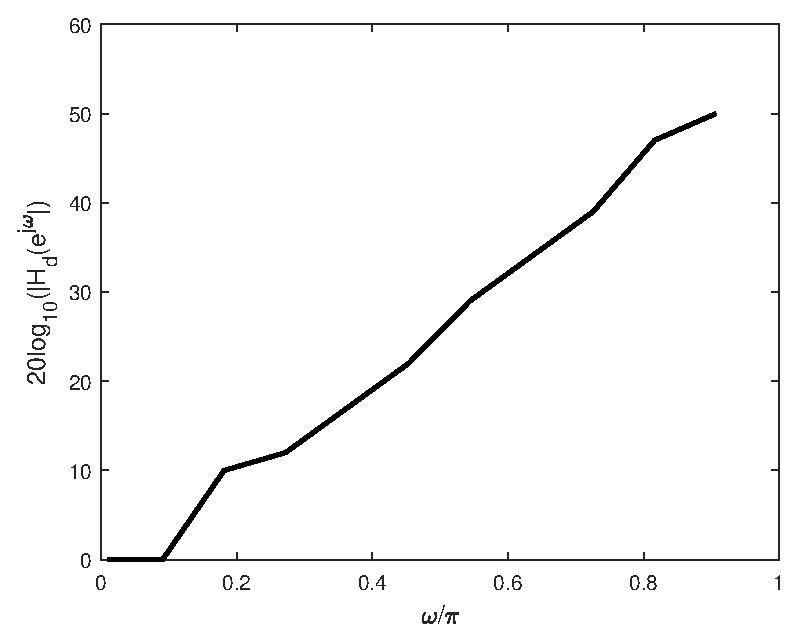
\includegraphics[scale=0.6]{figs/hearing_aid_spec.eps}
			\caption{Filter specification for correction of the patient's hearing loss.}
		\end{figure}
		\FloatBarrier
	}
	\fi
	
	\item (5 points) The reconstruction filter of the DAC is a linear interpolator. This filter has a continuous-time frequency response given by
	\begin{equation}
	H_{DAC}(j\Omega) = \mathrm{sinc}^2\Big(\frac{\Omega}{2\pi}T\Big), \quad |\Omega| \leq \frac{\pi}{T}.
	\end{equation}
	As a result, the reconstruction filter will cause some undesired attenuation in the band of interest from 0 to 10 kHz. Adjust the filter specification $|H_d(e^{j\omega})|$ calculated in part (a) so that the filter $H(z)$ would also compensate for the attenuation introduced by the DAC. Plot the adjusted specification. Once again, the $x$-axis of your plot should be normalized frequency $\omega$ or $\omega/\pi$, while the $y$-axis should be the magnitude $20\log_{10}(|H_d(e^{j\omega})|)$ in dB.
	
	\noindent\textit{Note:} In the DSP literature, pre-compensating for a filter response is called \textit{pre-emphasis}. In this question, you're performing pre-emphasis to compensate for the patient's hearing loss and also for the non-ideal reconstruction filter.
	
	\if\SOLUTIONS1
	{\color{\SolutionsColor} The corrected filter specification is given by
		\begin{equation*}
		|H_d(e^{j\omega})| = \frac{1}{|A(e^{j\omega})|\mathrm{sinc}^2(\frac{\omega}{2\pi})},
		\end{equation*}
		where $|A(e^{j\omega})|$ is patient's audiogram response. At the highest frequencies, the DAC causes about 8 dB of additional attenuation.
		
		\FloatBarrier
		\begin{figure}[h!]
			\centering
			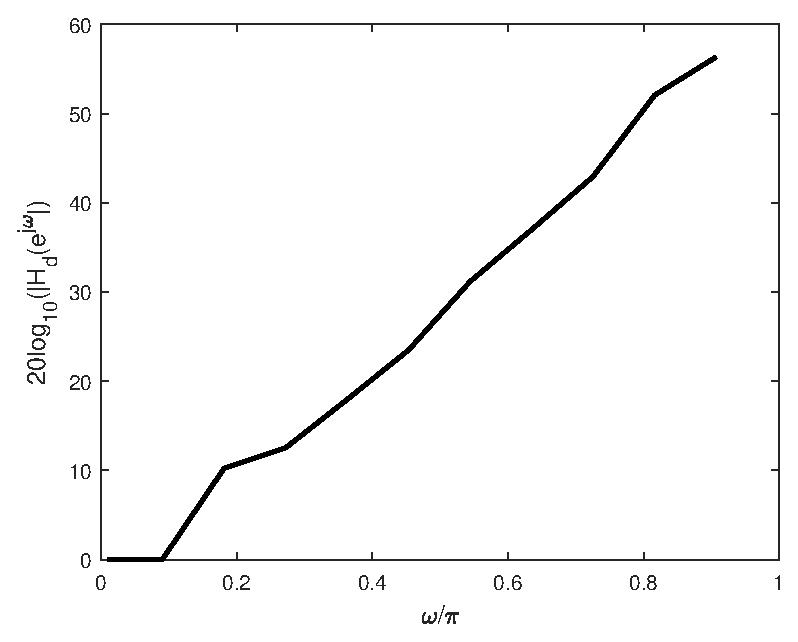
\includegraphics[scale=0.6]{figs/hearing_aid_corrected_spec.eps}
			\caption{Corrected filter specification that accounts for the DAC attenuation.}
		\end{figure}
		\FloatBarrier
	}
	\fi
	
	\item (15 points) Using your specification from part (b), design a generalized \underline{linear-phase} filter $H(z)$ that will approximate $|H_d(e^{j\omega})|$. Select the filter order so that the error between the desired response $H_d(e^{j\omega})$ and your design is \underline{at most} 1 dB at all frequencies. Plot $20\log_{10}(|H_d(e^{j\omega})|/|H(e^{j\omega})|)$ to show that your filter meets this specification. Additionally, plot the magnitude and phase response of your filter. 
	
	\if\SOLUTIONS1
	{\color{\SolutionsColor} Using the least-squares method, the filter that meets the specification to within 1 dB has order $M = 37$. Other answers obtained through the least-squares or Parks-McClellan method are accepted as long as the error is smaller than 1 dB at all frequencies.
		
		\FloatBarrier
		\begin{figure}[h!]
			\centering
			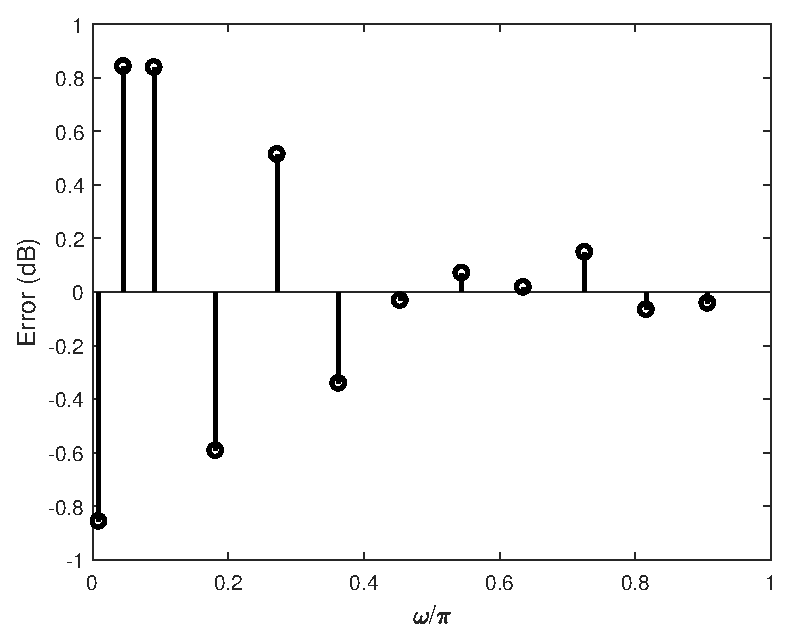
\includegraphics[scale=0.6]{figs/hearing_aid_filter_error.eps}
			\caption{Magnitude difference between the designed FIR filter and the specification from part (b). The error is smaller than 1 dB at all given frequencies. The filter order is $M = 37$.}
		\end{figure}
		\FloatBarrier	
		
		The frequency and phase response of filter is shown below
		\FloatBarrier
		\begin{figure}
			\centering
			\begin{subfigure}[h!]{0.5\textwidth}
				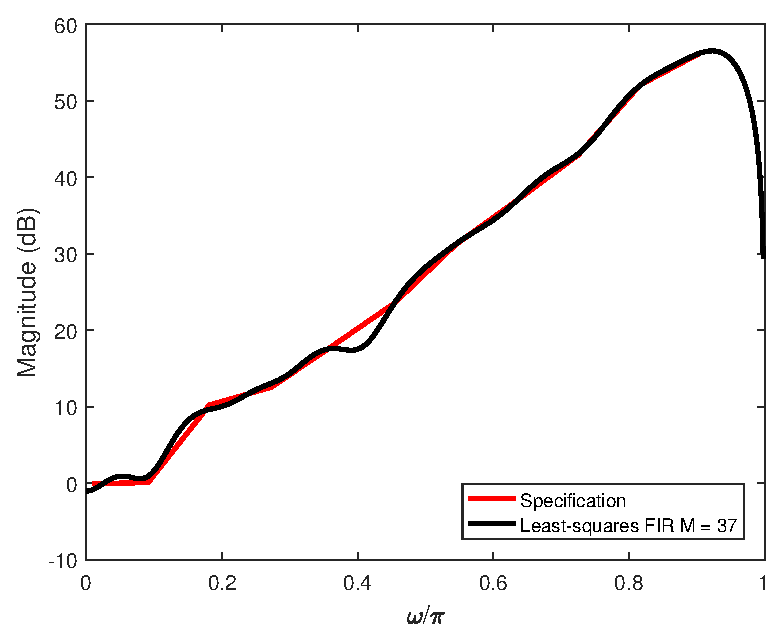
\includegraphics[scale=0.55]{figs/hearing_aid_filter_mag.eps}
				\caption{Magnitude}
			\end{subfigure}~\begin{subfigure}[h!]{0.5\textwidth}
				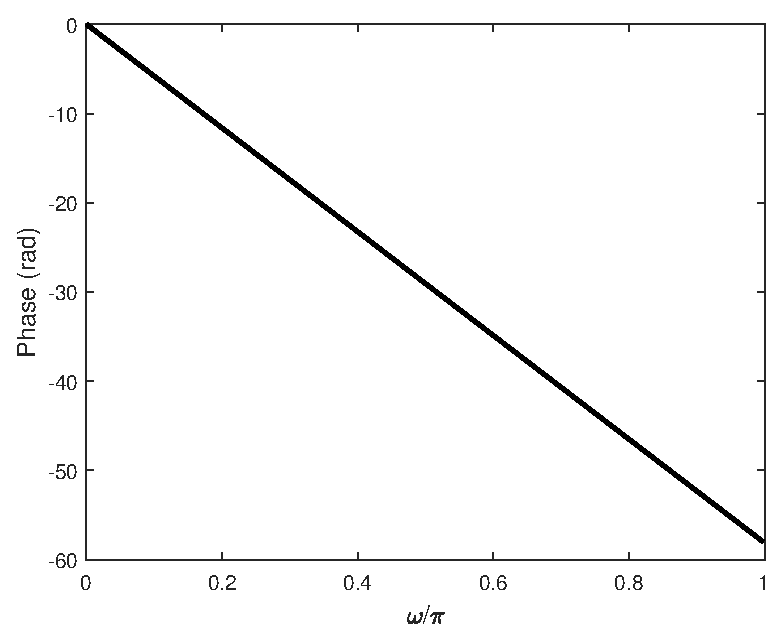
\includegraphics[scale=0.55]{figs/hearing_aid_filter_phase.eps}
				\caption{Phase}
			\end{subfigure}
			\caption{(a) magnitude and (b) phase of FIR filter of order $M = 37$ designed by the least-squares algorithm.}
		\end{figure}
		\FloatBarrier	
	}
	\fi
	
	\item (5 points) Assuming that your filter is the only cause of delay in the system, what is the time difference between the time that the sound is recorded by the microphone and the time it is outputted by the speaker. Give your answers in samples and in seconds. 
	
	\if\SOLUTIONS1 {\color{\SolutionsColor} Since the filter is linear phase, it has equal group delay at all frequencies. The group delay is
		\begin{equation*}
		n_g = \frac{M}{2} = 18.5~\text{samples} \implies \tau_g = Tn_g = 0.839~\text{ms}
		\end{equation*}	
	}\fi
	
	\item (10 points) Considering only quantization noise from the ADC, specify the minimum ADC resolution (in bits) so that the quantization noise average power \underline{after} $H(z)$ is at most $-30$ dBm (or 1 $\mu$W). Assume that the dynamic range of the quantizer is $\Delta X = 2$.
	
	\if\SOLUTIONS1 {\color{\SolutionsColor} Quantization noise has average power given by
		\begin{equation*}
		\sigma_Q^2 = \frac{\Delta^2}{12}, \quad \Delta = \frac{\Delta X}{2^B}
		\end{equation*}
		
		However, quantization noise is shaped by the filter $H(z)$. The noise average power after filtering is given by
		\begin{equation*}
		\sigma^2_{Q, out} = \sigma_Q^2\sum_{n = 0}^{M}|h[n]|^2 \tag{quantization noise shaping}
		\end{equation*}
		
		The output noise average power is smaller than $-30$ dBm (or $1 \mu$W) when $B = 18$, as can be verified in the plot below
		
		\FloatBarrier
		\begin{figure}[h!]
			\centering
			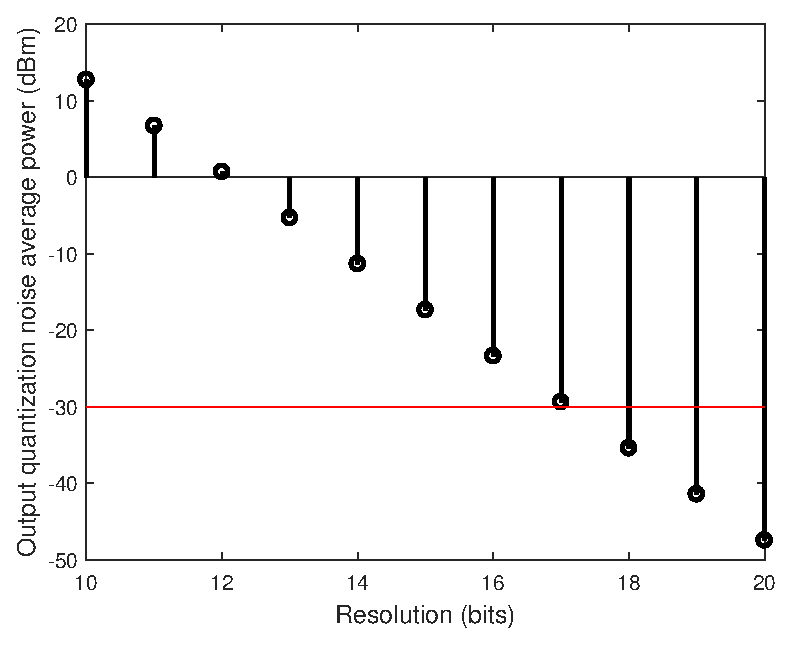
\includegraphics[scale=0.6]{figs/hearing_aid_quant_noise_var.eps}
			\caption{Average power of output quantization noise as a function of the resolution of the quantizer.}
		\end{figure}
		\FloatBarrier	
		
		Slightly different results may be obtained for different filters.
	}\fi
	
	\item (10 points) Now include round-off noise from the filter implementation and determine the minimum ADC resolution (in bits) so that the \underline{total noise power} after $H(z)$ is at most $-30$ dBm (or 1 $\mu$W). Assume that the filter is implemented using the direct form I, and calculations are performed in two's complement using Q($B-1$) representation, where $B$ is the resolution of the ADC quantizer. Assume further that the result of multiplications is quantized \underline{immediately before} any additions are done. For the roundoff noise calculations assume that $X_m = 1$.
	
	\noindent\textit{Note:} Recall that in linear-phase implementations not all the coefficients need to be multiplied because of the symmetry in the impulse response.
	
	\if\SOLUTIONS1 {\color{\SolutionsColor} The number of required multiplications in a linear phase FIR filter is $\lfloor \frac{M}{2} + 1 \rfloor$. Therefore, the round-off noise resulting from rounding off the numbers immediately before additions is given by
		\begin{equation*}
		\sigma_{roundoff}^2 = \Big\lfloor \frac{M}{2} + 1 \Big\rfloor\frac{\Delta^2}{12}, \quad\Delta = \frac{X_m}{2^{B-1}}
		\end{equation*}
		Note that we use $B-1$ because the problem statement instructs us to use the Q($B-1$) representation, where $B$ is the number of bits of the ADC. In the lecture notes of roundoff noise, the quantizer had $B+1$ bits and we used the Q$B$ representation for numbers in the $[-1, 1]$ interval. 
		
		The roundoff noise is not shaped by the filter, hence the total noise average power after the $H(z)$ is given by
		\begin{equation*}
		\sigma^2_{total} = \sigma_Q^2\sum_{n = 0}^{M}|h[n]|^2 + \sigma_{roundoff}^2
		\end{equation*}
		
		The total noise average power after $H(z)$ is smaller than $-30$ dBm (or $1 \mu$W) when $B = 18$, as can be verified in the plot below
		
		\FloatBarrier
		\begin{figure}[h!]
			\centering
			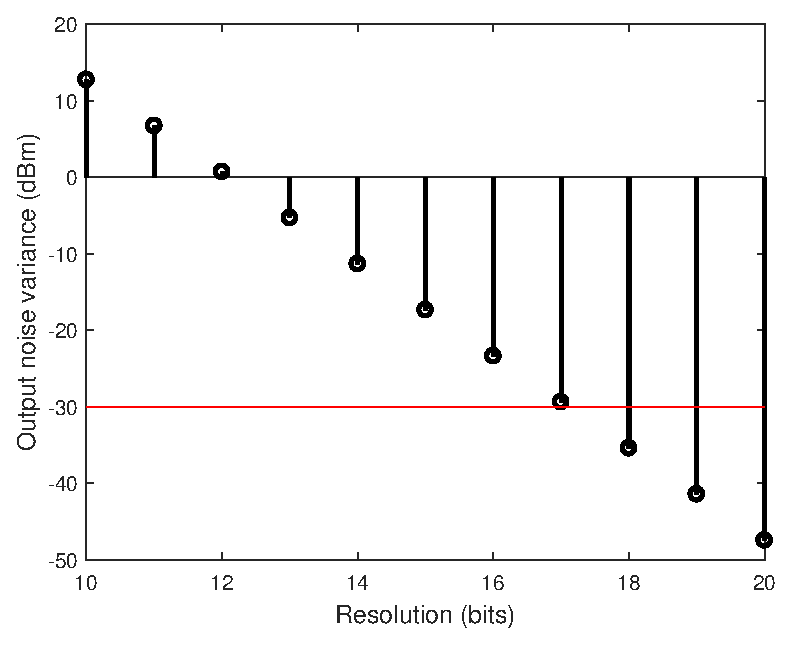
\includegraphics[scale=0.6]{figs/hearing_aid_total_noise_var.eps}
			\caption{Total noise average power after $H(z)$ as a function of the resolution of the quantizer.}
		\end{figure}
		\FloatBarrier
		
		Slightly different results may be obtained for different filters.
	}\fi
	
	
	\item (10 points) Now perform simulations to check whether your noise calculations are correct. In your simulations, you should include one white noise source to model quantization noise, and another white noise source to model round-off noise. These noise sources have to be \underline{zero mean} and have the appropriate \underline{average power}. Using any technique you prefer, estimate the PSD of the \underline{total noise} at the output of $H(z)$. On the same graph, plot the theoretical PSD and the estimated PSD. Use your result to estimate the average power of the noise and discuss whether it agrees with your theoretical estimates of part (e).
	
	\noindent\textit{Note:} Use the function \texttt{rand} to generate a white uniformly distributed noise, and use \texttt{filter} to filter the noise. Make sure that your noise sources are \underline{zero mean} and have the correct \underline{average power}.
	
	\if\SOLUTIONS1 {\color{\SolutionsColor}
		For the quantization noise, we need to generate an uniformly distributed zero-mean white noise signal with average power $\sigma_Q^2$, as calculated in part (e). For the roundoff noise, we need to generate an uniformly distributed zero-mean white noise signal with average power $\sigma_{roundoff}^2$, as calculated in part (f). The total noise will be given by
		\begin{equation}
		y[n] = h[n]\ast q[n] + r[n],
		\end{equation}
		where $q[n]$ is the quantization noise and $r[n]$ is the roundoff noise. Once we obtain the output noise $y[n]$ we can use Welch's method or the Blackman-Tukey method to estimate the PSD. These solutions assume the Blackman-Tukey method with Bartlett window of length $L = 2047$. See code for more details. The estimated PSD is plotted below
		
		\FloatBarrier
		\begin{figure}[h!]
			\centering
			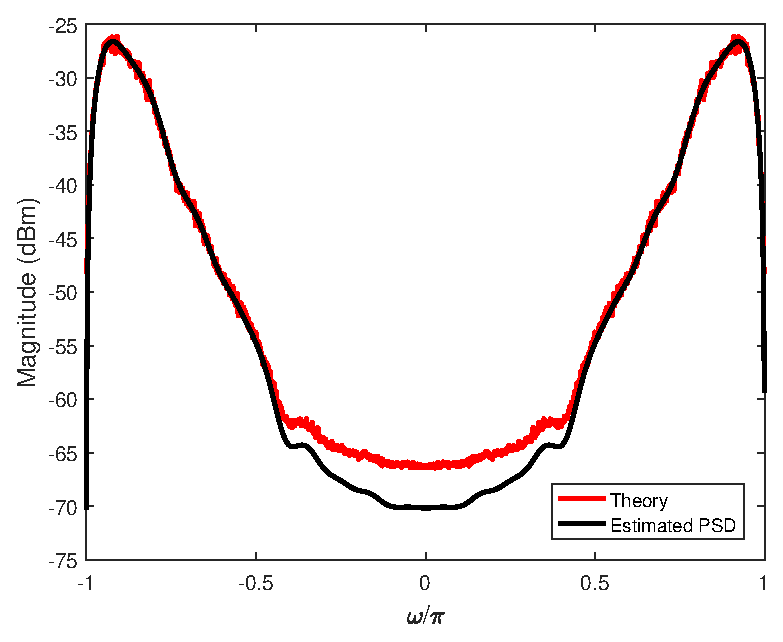
\includegraphics[scale=0.6]{figs/hearing_aid_psd.eps}
			\caption{Theoretical and estimated PSD. The PSD was estimated using the Blackman-Tukey method.}
		\end{figure}
		\FloatBarrier
		
		Note the error of the estimated PSD at small frequencies. To improve the accuracy we would need more samples. However, this error is not important, since the estimated power is nearly identical to the theoretical power. The estimated power is $-35.4977$. Hence, this design meets the specifications.
	}\fi
	
\end{enumerate}

\if\SOLUTIONS1 
\subsection*{Code for Problem 1}
% This file was automatically created from the m-file 
% "m2tex.m" written by USL. 
% The fontencoding in this file is UTF-8. 
%  
% You will need to include the following two packages in 
% your LaTeX-Main-File. 
%  
% \usepackage{color} 
% \usepackage{fancyvrb} 
%  
% It is advised to use the following option for Inputenc 
% \usepackage[utf8]{inputenc} 
%  
  
% definition of matlab colors: 
\definecolor{mblue}{rgb}{0,0,1} 
\definecolor{mgreen}{rgb}{0.13333,0.5451,0.13333} 
\definecolor{mred}{rgb}{0.62745,0.12549,0.94118} 
\definecolor{mgrey}{rgb}{0.5,0.5,0.5} 
\definecolor{mdarkgrey}{rgb}{0.25,0.25,0.25} 
  
\DefineShortVerb[fontfamily=courier,fontseries=m]{\$} 
\DefineShortVerb[fontfamily=courier,fontseries=b]{\#} 
  
\noindent                                                                                                                                              
 \hspace*{-1.6em}{\scriptsize 1}$  $\color{mgrey}#%% Hearing aid problem #\color{black}$$\\
 \hspace*{-1.6em}{\scriptsize 2}$  clear, $\color{mdarkgrey}$clc, close all$\color{black}$$\\
 \hspace*{-1.6em}{\scriptsize 3}$  $\\
 \hspace*{-1.6em}{\scriptsize 4}$  T = 1/22.05e3;     $\color{mgrey}$% sampling time in seconds$\color{black}$$\\
 \hspace*{-1.6em}{\scriptsize 5}$  f = 1e3*[0.1 0.5 1 2 3 4 5 6 7 8 9 10]; $\color{mgrey}$% in Hz$\color{black}$$\\
 \hspace*{-1.6em}{\scriptsize 6}$  A = [0 0 0 -10 -12 -17 -22 -29 -34 -39 -47 -50]; $\color{mgrey}$% in dB$\color{black}$$\\
 \hspace*{-1.6em}{\scriptsize 7}$  $\\
 \hspace*{-1.6em}{\scriptsize 8}$  $\color{mgrey}#%% a)#\color{black}$$\\
 \hspace*{-1.6em}{\scriptsize 9}$  w_spec = 2*pi*f*T;$\\
 \hspace*{-2em}{\scriptsize 10}$  $\\
 \hspace*{-2em}{\scriptsize 11}$  $\color{mgrey}$% Plot results$\color{black}$$\\
 \hspace*{-2em}{\scriptsize 12}$  figure, $\color{mdarkgrey}$box on$\color{black}$$\\
 \hspace*{-2em}{\scriptsize 13}$  plot(w_spec/pi, -A, $\color{mdarkgrey}$'k'$\color{black}$, $\color{mdarkgrey}$'LineWidth'$\color{black}$, 2)$\\
 \hspace*{-2em}{\scriptsize 14}$  xlabel($\color{mdarkgrey}$'\omega/\pi'$\color{black}$, $\color{mdarkgrey}$'FontSize'$\color{black}$, 12)$\\
 \hspace*{-2em}{\scriptsize 15}$  ylabel($\color{mdarkgrey}$'20log_{10}(|H_d(e^{j\omega}|)'$\color{black}$, $\color{mdarkgrey}$'FontSize'$\color{black}$, 12)$\\
 \hspace*{-2em}{\scriptsize 16}$  axis([0 $\color{mdarkgrey}$1 0 60])$\color{black}$$\\
 \hspace*{-2em}{\scriptsize 17}$  saveas(gca, $\color{mdarkgrey}$'../figs/hearing_aid_spec'$\color{black}$, $\color{mdarkgrey}$'epsc'$\color{black}$)$\\
 \hspace*{-2em}{\scriptsize 18}$      $\\
 \hspace*{-2em}{\scriptsize 19}$  $\color{mgrey}#%% b)#\color{black}$$\\
 \hspace*{-2em}{\scriptsize 20}$  Hd = 1./(10.^(A/20).*sinc(w_spec/(2*pi)).^2);$\\
 \hspace*{-2em}{\scriptsize 21}$  figure, $\color{mdarkgrey}$plot(w_spec/pi, 20*log10(abs(Hd)))$\color{black}$$\\
 \hspace*{-2em}{\scriptsize 22}$  $\\
 \hspace*{-2em}{\scriptsize 23}$  $\color{mgrey}$% Plot results$\color{black}$$\\
 \hspace*{-2em}{\scriptsize 24}$  figure, $\color{mdarkgrey}$box on$\color{black}$$\\
 \hspace*{-2em}{\scriptsize 25}$  plot(w_spec/pi, 20*log10(abs(Hd)), $\color{mdarkgrey}$'k'$\color{black}$, $\color{mdarkgrey}$'LineWidth'$\color{black}$, 2)$\\
 \hspace*{-2em}{\scriptsize 26}$  xlabel($\color{mdarkgrey}$'\omega/\pi'$\color{black}$, $\color{mdarkgrey}$'FontSize'$\color{black}$, 12)$\\
 \hspace*{-2em}{\scriptsize 27}$  ylabel($\color{mdarkgrey}$'20log_{10}(|H_d(e^{j\omega}|)'$\color{black}$, $\color{mdarkgrey}$'FontSize'$\color{black}$, 12)$\\
 \hspace*{-2em}{\scriptsize 28}$  axis([0 $\color{mdarkgrey}$1 0 60])$\color{black}$$\\
 \hspace*{-2em}{\scriptsize 29}$  saveas(gca, $\color{mdarkgrey}$'../figs/hearing_aid_corrected_spec'$\color{black}$, $\color{mdarkgrey}$'epsc'$\color{black}$)$\\
 \hspace*{-2em}{\scriptsize 30}$  $\\
 \hspace*{-2em}{\scriptsize 31}$  $\color{mgrey}#%% c)#\color{black}$$\\
 \hspace*{-2em}{\scriptsize 32}$  $#for#$ M = 2:100$\\
 \hspace*{-2em}{\scriptsize 33}$      hls = firls(M, w_spec/pi, Hd); $\color{mgrey}$% design filter of order M$\color{black}$$\\
 \hspace*{-2em}{\scriptsize 34}$      error = 20*log10(abs(freqz(hls, 1, w_spec))./abs(Hd));$\\
 \hspace*{-2em}{\scriptsize 35}$      $#if#$ all(abs(error) < 1) $\color{mgrey}$% error is smaller than 1 dB at all frequencies$\color{black}$$\\
 \hspace*{-2em}{\scriptsize 36}$          $#break#$$\\
 \hspace*{-2em}{\scriptsize 37}$      $#end#$$\\
 \hspace*{-2em}{\scriptsize 38}$  $#end#$$\\
 \hspace*{-2em}{\scriptsize 39}$  $\\
 \hspace*{-2em}{\scriptsize 40}$  M $\color{mgrey}$% filter order that meets specs$\color{black}$$\\
 \hspace*{-2em}{\scriptsize 41}$  [Hls, $\color{mdarkgrey}$w] = freqz(hls, 1);$\color{black}$$\\
 \hspace*{-2em}{\scriptsize 42}$  $\\
 \hspace*{-2em}{\scriptsize 43}$  $\color{mgrey}$% Plot results$\color{black}$$\\
 \hspace*{-2em}{\scriptsize 44}$  figure, $\color{mdarkgrey}$hold on, box on$\color{black}$$\\
 \hspace*{-2em}{\scriptsize 45}$  stem(w_spec/pi, 20*log10(abs(freqz(hls, 1, w_spec))./abs(Hd)), $\color{mdarkgrey}$'k'$\color{black}$, $\color{mdarkgrey}$'LineWidth'$\color{black}$, 2)$\\
 \hspace*{-2em}{\scriptsize 46}$  xlabel($\color{mdarkgrey}$'\omega/\pi'$\color{black}$, $\color{mdarkgrey}$'FontSize'$\color{black}$, 12)$\\
 \hspace*{-2em}{\scriptsize 47}$  ylabel($\color{mdarkgrey}$'Error (dB)'$\color{black}$, $\color{mdarkgrey}$'FontSize'$\color{black}$, 12)$\\
 \hspace*{-2em}{\scriptsize 48}$  axis([0 $\color{mdarkgrey}$1 -1 1])$\color{black}$$\\
 \hspace*{-2em}{\scriptsize 49}$  saveas(gca, $\color{mdarkgrey}$'../figs/hearing_aid_filter_error'$\color{black}$, $\color{mdarkgrey}$'epsc'$\color{black}$)$\\
 \hspace*{-2em}{\scriptsize 50}$  $\\
 \hspace*{-2em}{\scriptsize 51}$  figure, $\color{mdarkgrey}$hold on, box on$\color{black}$$\\
 \hspace*{-2em}{\scriptsize 52}$  plot(w_spec/pi, 20*log10(abs(Hd)), $\color{mdarkgrey}$'r'$\color{black}$, $\color{mdarkgrey}$'LineWidth'$\color{black}$, 2)$\\
 \hspace*{-2em}{\scriptsize 53}$  plot(w/pi, 20*log10(abs(Hls)), $\color{mdarkgrey}$'k'$\color{black}$, $\color{mdarkgrey}$'LineWidth'$\color{black}$, 2)$\\
 \hspace*{-2em}{\scriptsize 54}$  legend($\color{mdarkgrey}$'Specification'$\color{black}$, sprintf($\color{mdarkgrey}$'Least-squares FIR M = %d'$\color{black}$, M),...$\\
 \hspace*{-2em}{\scriptsize 55}$      $\color{mdarkgrey}$'Location'$\color{black}$, $\color{mdarkgrey}$'SouthEast'$\color{black}$)$\\
 \hspace*{-2em}{\scriptsize 56}$  xlabel($\color{mdarkgrey}$'\omega/\pi'$\color{black}$, $\color{mdarkgrey}$'FontSize'$\color{black}$, 12)$\\
 \hspace*{-2em}{\scriptsize 57}$  ylabel($\color{mdarkgrey}$'Magnitude (dB)'$\color{black}$, $\color{mdarkgrey}$'FontSize'$\color{black}$, 12)$\\
 \hspace*{-2em}{\scriptsize 58}$  saveas(gca, $\color{mdarkgrey}$'../figs/hearing_aid_filter_mag'$\color{black}$, $\color{mdarkgrey}$'epsc'$\color{black}$)$\\
 \hspace*{-2em}{\scriptsize 59}$  $\\
 \hspace*{-2em}{\scriptsize 60}$  figure, $\color{mdarkgrey}$box on$\color{black}$$\\
 \hspace*{-2em}{\scriptsize 61}$  plot(w/pi, unwrap(angle(Hls)), $\color{mdarkgrey}$'k'$\color{black}$, $\color{mdarkgrey}$'LineWidth'$\color{black}$, 2)$\\
 \hspace*{-2em}{\scriptsize 62}$  xlabel($\color{mdarkgrey}$'\omega/\pi'$\color{black}$, $\color{mdarkgrey}$'FontSize'$\color{black}$, 12)$\\
 \hspace*{-2em}{\scriptsize 63}$  ylabel($\color{mdarkgrey}$'Phase (rad)'$\color{black}$, $\color{mdarkgrey}$'FontSize'$\color{black}$, 12)$\\
 \hspace*{-2em}{\scriptsize 64}$  saveas(gca, $\color{mdarkgrey}$'../figs/hearing_aid_filter_phase'$\color{black}$, $\color{mdarkgrey}$'epsc'$\color{black}$)$\\
 \hspace*{-2em}{\scriptsize 65}$  $\\
 \hspace*{-2em}{\scriptsize 66}$  $\color{mgrey}#%% d)#\color{black}$$\\
 \hspace*{-2em}{\scriptsize 67}$  delay_samples = M/2 $\color{mgrey}$% delay of linear phase filter$\color{black}$$\\
 \hspace*{-2em}{\scriptsize 68}$  delay_time = delay_samples*T$\\
 \hspace*{-2em}{\scriptsize 69}$  $\\
 \hspace*{-2em}{\scriptsize 70}$  $\color{mgrey}#%% e)#\color{black}$$\\
 \hspace*{-2em}{\scriptsize 71}$  $\color{mgrey}$% Quantization noise power$\color{black}$$\\
 \hspace*{-2em}{\scriptsize 72}$  DeltaX = 2;$\\
 \hspace*{-2em}{\scriptsize 73}$  B = 10:20;$\\
 \hspace*{-2em}{\scriptsize 74}$  Delta = DeltaX./2.^B;$\\
 \hspace*{-2em}{\scriptsize 75}$  varQ = Delta.^2/12;$\\
 \hspace*{-2em}{\scriptsize 76}$  $\\
 \hspace*{-2em}{\scriptsize 77}$  varQuant = varQ*sum(abs(hls).^2);$\\
 \hspace*{-2em}{\scriptsize 78}$  $\\
 \hspace*{-2em}{\scriptsize 79}$  $\color{mgrey}$% Plot results$\color{black}$$\\
 \hspace*{-2em}{\scriptsize 80}$  figure, $\color{mdarkgrey}$box on, hold on$\color{black}$$\\
 \hspace*{-2em}{\scriptsize 81}$  stem(B, 10*log10(varQuant/1e-3), $\color{mdarkgrey}$'k'$\color{black}$, $\color{mdarkgrey}$'LineWidth'$\color{black}$, 2)$\\
 \hspace*{-2em}{\scriptsize 82}$  plot([B(1) B(end)], [-30 -30], $\color{mdarkgrey}$'r'$\color{black}$)$\\
 \hspace*{-2em}{\scriptsize 83}$  xlabel($\color{mdarkgrey}$'Resolution (bits)'$\color{black}$, $\color{mdarkgrey}$'FontSize'$\color{black}$, 12)$\\
 \hspace*{-2em}{\scriptsize 84}$  ylabel($\color{mdarkgrey}$'Output quantization noise average power (dBm)'$\color{black}$, $\color{mdarkgrey}$'FontSize'$\color{black}$, 12)$\\
 \hspace*{-2em}{\scriptsize 85}$  saveas(gca, $\color{mdarkgrey}$'../figs/hearing_aid_quant_noise_var'$\color{black}$, $\color{mdarkgrey}$'epsc'$\color{black}$)$\\
 \hspace*{-2em}{\scriptsize 86}$  $\\
 \hspace*{-2em}{\scriptsize 87}$  $\color{mgrey}#%% f)#\color{black}$$\\
 \hspace*{-2em}{\scriptsize 88}$  $\color{mgrey}$% Roundoff noise$\color{black}$$\\
 \hspace*{-2em}{\scriptsize 89}$  Nmult = floor(M/2+1);$\\
 \hspace*{-2em}{\scriptsize 90}$  $\\
 \hspace*{-2em}{\scriptsize 91}$  $\color{mgrey}$% Rounoff noise is not enhanced by filter$\color{black}$$\\
 \hspace*{-2em}{\scriptsize 92}$  varRoundOff = Nmult*(1./(2.^(B-1))).^2/12;$\\
 \hspace*{-2em}{\scriptsize 93}$  $\\
 \hspace*{-2em}{\scriptsize 94}$  $\color{mgrey}$% Plot results$\color{black}$$\\
 \hspace*{-2em}{\scriptsize 95}$  figure, $\color{mdarkgrey}$box on, hold on$\color{black}$$\\
 \hspace*{-2em}{\scriptsize 96}$  stem(B, 10*log10((varRoundOff + varQuant)/1e-3), $\color{mdarkgrey}$'k'$\color{black}$, $\color{mdarkgrey}$'LineWidth'$\color{black}$, 2)$\\
 \hspace*{-2em}{\scriptsize 97}$  plot([B(1) B(end)], [-30 -30], $\color{mdarkgrey}$'r'$\color{black}$)$\\
 \hspace*{-2em}{\scriptsize 98}$  xlabel($\color{mdarkgrey}$'Resolution (bits)'$\color{black}$, $\color{mdarkgrey}$'FontSize'$\color{black}$, 12)$\\
 \hspace*{-2em}{\scriptsize 99}$  ylabel($\color{mdarkgrey}$'Output noise variance (dBm)'$\color{black}$, $\color{mdarkgrey}$'FontSize'$\color{black}$, 12)$\\
 \hspace*{-2.4em}{\scriptsize 100}$  saveas(gca, $\color{mdarkgrey}$'../figs/hearing_aid_total_noise_var'$\color{black}$, $\color{mdarkgrey}$'epsc'$\color{black}$)$\\
 \hspace*{-2.4em}{\scriptsize 101}$  $\\
 \hspace*{-2.4em}{\scriptsize 102}$  $\color{mgrey}#%% g)#\color{black}$$\\
 \hspace*{-2.4em}{\scriptsize 103}$  B = 18;$\\
 \hspace*{-2.4em}{\scriptsize 104}$  Delta = DeltaX/2^B;$\\
 \hspace*{-2.4em}{\scriptsize 105}$  varQ = Delta^2/12;$\\
 \hspace*{-2.4em}{\scriptsize 106}$  varRoundOff = Nmult*(1/(2^(B-1)))^2/12;$\\
 \hspace*{-2.4em}{\scriptsize 107}$  $\\
 \hspace*{-2.4em}{\scriptsize 108}$  $\color{mgrey}$% $\color{black}$$\\
 \hspace*{-2.4em}{\scriptsize 109}$  q = sqrt(varQ)/sqrt(1/12)*(rand(1, 10e4)-0.5); $\color{mgrey}$% quantization noise$\color{black}$$\\
 \hspace*{-2.4em}{\scriptsize 110}$  roundoff = sqrt(varRoundOff)/sqrt(1/12)*(rand(1, 10e4)-0.5); $\color{mgrey}$% roundoff noise$\color{black}$$\\
 \hspace*{-2.4em}{\scriptsize 111}$  $\\
 \hspace*{-2.4em}{\scriptsize 112}$  $\color{mgrey}$% Quantization noise is shaped by the filter, but roundoff noise is not $\color{black}$$\\
 \hspace*{-2.4em}{\scriptsize 113}$  noise = filter(hls, 1, q) + roundoff;$\\
 \hspace*{-2.4em}{\scriptsize 114}$  $\\
 \hspace*{-2.4em}{\scriptsize 115}$  $\color{mgrey}$% PSD estimation$\color{black}$$\\
 \hspace*{-2.4em}{\scriptsize 116}$  M = 1024;$\\
 \hspace*{-2.4em}{\scriptsize 117}$  L = 2*M-1;$\\
 \hspace*{-2.4em}{\scriptsize 118}$  window = bartlett(L).';$\\
 \hspace*{-2.4em}{\scriptsize 119}$  dw = 2*pi/L;$\\
 \hspace*{-2.4em}{\scriptsize 120}$  w = -pi:dw:pi-dw; $\color{mgrey}$% frequency vector$\color{black}$$\\
 \hspace*{-2.4em}{\scriptsize 121}$  $\\
 \hspace*{-2.4em}{\scriptsize 122}$  Pw = blackman_tukey_psd(noise, window, M);$\\
 \hspace*{-2.4em}{\scriptsize 123}$  $\\
 \hspace*{-2.4em}{\scriptsize 124}$  $\color{mgrey}$% Average power estimation$\color{black}$$\\
 \hspace*{-2.4em}{\scriptsize 125}$  estimatedNoisePower = trapz(w, Pw)/(2*pi);$\\
 \hspace*{-2.4em}{\scriptsize 126}$  estimatedNoisePowerdBm = 10*log10(estimatedNoisePower/1e-3)$\\
 \hspace*{-2.4em}{\scriptsize 127}$  $\\
 \hspace*{-2.4em}{\scriptsize 128}$  $\color{mgrey}$% Theoretical PSD$\color{black}$$\\
 \hspace*{-2.4em}{\scriptsize 129}$  Hls = freqz(hls, 1, w);$\\
 \hspace*{-2.4em}{\scriptsize 130}$  Ptheory = varQ*abs(Hls).^2 + varRoundOff;$\\
 \hspace*{-2.4em}{\scriptsize 131}$  $\\
 \hspace*{-2.4em}{\scriptsize 132}$  theoreticalNoisePower = trapz(w, Pw)/(2*pi);$\\
 \hspace*{-2.4em}{\scriptsize 133}$  theoreticalNoisePowerdBm = 10*log10(theoreticalNoisePower/1e-3)$\\
 \hspace*{-2.4em}{\scriptsize 134}$  $\\
 \hspace*{-2.4em}{\scriptsize 135}$  $\color{mgrey}$% Plot results$\color{black}$$\\
 \hspace*{-2.4em}{\scriptsize 136}$  figure, $\color{mdarkgrey}$box on, hold on$\color{black}$$\\
 \hspace*{-2.4em}{\scriptsize 137}$  plot(w/pi, 10*log10(Pw/1e-3), $\color{mdarkgrey}$'r'$\color{black}$, $\color{mdarkgrey}$'LineWidth'$\color{black}$, 2)$\\
 \hspace*{-2.4em}{\scriptsize 138}$  plot(w/pi, 10*log10(Ptheory/1e-3), $\color{mdarkgrey}$'k'$\color{black}$, $\color{mdarkgrey}$'LineWidth'$\color{black}$, 2)$\\
 \hspace*{-2.4em}{\scriptsize 139}$  legend($\color{mdarkgrey}$'Theory'$\color{black}$, $\color{mdarkgrey}$'Estimated PSD'$\color{black}$, $\color{mdarkgrey}$'Location'$\color{black}$, $\color{mdarkgrey}$'SouthEast'$\color{black}$)$\\
 \hspace*{-2.4em}{\scriptsize 140}$  xlabel($\color{mdarkgrey}$'\omega/\pi'$\color{black}$, $\color{mdarkgrey}$'FontSize'$\color{black}$, 12)$\\
 \hspace*{-2.4em}{\scriptsize 141}$  ylabel($\color{mdarkgrey}$'Magnitude (dBm)'$\color{black}$, $\color{mdarkgrey}$'FontSize'$\color{black}$, 12)$\\
 \hspace*{-2.4em}{\scriptsize 142}$  saveas(gca, $\color{mdarkgrey}$'../figs/hearing_aid_psd'$\color{black}$, $\color{mdarkgrey}$'epsc'$\color{black}$)$\\ 
  
\UndefineShortVerb{\$} 
\UndefineShortVerb{\#}
\fi

\newpage

\section*{Problem 2: Nonlinear plant identification (60 points)}

As discussed in class, we can use adaptive filters to model unknown plants. In many practical applications, however, the plant may exhibit some nonlinear characteristic that cannot be accurately modeled by linear filtering alone. In this question, you'll design and compare linear and nonlinear adaptive filters to model a given nonlinear plant.

The typical block diagram of plant identification problems is shown in Figure~\ref{fig:block-diagram}. An input signal $r[n]$ is presented to the plant and to the adaptive filter. The output of the plant $d[n]$ is the desired response that we use to compute the error $e[n]$. As usual, the output of the adaptive filter $y[n]$ is expressed as the inner product of an input vector $X_n$ and the weight vector $W$. In a linear adaptive filter, the input vector depends only on linear or affine terms of the input $r[n]$, whereas in a nonlinear adaptive filter, the input vector also contains some nonlinear terms of the input $r[n]$.

\begin{figure}[h!]
	\flushleft
	\resizebox{\linewidth}{!}{\def\layersep{1.5cm}
\def\outsep{0.7cm}
\def\dy{1.25}

\begin{tikzpicture}[->, >=stealth, shorten >= 0pt, draw=black!50, node distance=\layersep, font=\sffamily]
\tikzstyle{node}=[circle,fill=black,minimum size=2pt,inner sep=0pt]
\tikzstyle{weight}=[draw=black,circle,fill=none,minimum size=3pt,inner sep=0pt,font=\fontsize{6}{6}\selectfont]
\tikzstyle{summer}=[weight, minimum size=15pt, inner sep=2pt]
\tikzstyle{block}=[draw=black,rectangle,fill=none,minimum size=1cm, inner sep=0pt]
\tikzstyle{annot} = []

\node[node] (rk) at (0, -\dy cm) {};
\node[node] (in) at (0.25*\layersep, -\dy cm) {};
\node[block] (H1) at (1*\layersep, -\dy cm) {$H_1(z)$};
\node[block] (g) at (2*\layersep, -\dy cm) {$g(\cdot)$};
\node[block] (H2) at (3*\layersep, -\dy cm) {$H_2(z)$};
\draw[-, dashed] (1*\layersep-0.75cm,-\dy*0.5) rectangle (3*\layersep+0.75cm,-1.5*\dy);
\node[annot, below=4pt] at (2*\layersep, -1.5*\dy) {``Unknown'' plant};
\node[node] (plant-out) at (4*\layersep, -\dy cm) {};
\coordinate (output) at (4.5*\layersep, -\dy cm) {};
\node[summer] (error) at (4*\layersep, -2*\dy cm) {\Large $\Sigma$};
\coordinate (error-out) at (4.5*\layersep, -2*\dy cm) {};

\draw (error-out) -- (4.5*\layersep, -3.75*\dy cm) -- (2.5*\layersep, -3.75*\dy cm) -- (1.5*\layersep, -2.3*\dy cm);
\node[block, fill=white, minimum width=3cm] (adapt) at (2*\layersep, -3*\dy cm) {Adaptive filter};

\path[-] (rk) edge (in);
\path (in) edge (H1);
\path (H1) edge (g);
\path (g) edge (H2);
\path[-] (H2) edge (plant-out);
\draw (in) |- (adapt);
\draw (plant-out) -- (output);
\draw (plant-out) -- (error);
\draw[-] (error) -- (error-out);
\draw (adapt) -| (error);

\node[above right = 0.5mm and 0.1mm of error, scale=0.8] {$+$};
\node[below right = 0.5mm and 0.1mm of error, scale=0.8] {$-$};
\node[left = -2mm of rk, text width = 2cm, align=center, scale=0.8] {Plant input \\ $r[n]$};
\node[right = -2mm of output, text width = 3cm, align=center, scale=0.8] {Desired response \\ $d[n]$};
\node[scale=0.8, below right = -5mm and 1mm of adapt] {$y[n] = X_n^TW$};
\node[right = 1mm of error-out, align=center, scale=0.8] {error \\ $e[n]$};



% 	\node[summer] (Adder) at (3*\layersep,-\dy*2.5 cm) {\large $\Sigma$}; 
%     \node[node, inner sep=0pt] (mid) at (4.5*\layersep,-\dy*2.5 cm) {}; 

%     \node[node, inner sep=0pt] (output-tap) at (7.3*\layersep,-\dy*2.5 cm) {};
%     \coordinate (output) at (8*\layersep,-\dy*2.5 cm) {};
%     \node[summer, minimum size=10pt] (error) at (6*\layersep,-\dy*5 cm) {$\Sigma$}; 
%     \coordinate (xw) at (4.5*\layersep,-\dy*5 cm) {};
%     \coordinate (out) at (7.3*\layersep,-\dy*5 cm) {};
%     \node[weight,fill=white] (gamma) at (4.5*\layersep,-\dy*4 cm) {\small $\gamma$};
%     \coordinate (error-out) at (6*\layersep,-\dy*6 cm) {};


%     \coordinate (A) at (\layersep,-6*\dy cm) {};
%     \coordinate (B) at (\layersep,\dy cm) {};
%     \path (A) edge (B);
%     \path[-] (error) edge (error-out);
%     \path[-] (error-out) edge (A);

%     \foreach \name / \y in {0,...,3} {
%     % This is the same as writing \foreach \name / \y in {1/1,2/2,3/3,4/4}
%         \node[node] (I-\name) at (0,-\dy*\y) {}; % Draw the input layer nodes
%         \node[weight,fill=white] (W-\name) at (\layersep,-\dy*\y cm) {$W_\name$}; % Draw the hidden layer  layer node     
%      }   	

% 	\node[node] (I-4) at (0,-5*\dy cm) {}; % Draw the hidden layer 
% 	\node[weight, fill=white] (W-4) at (\layersep,-5*\dy cm) {$W_n$};

%     %% Annotations
%     \node[annot] at (-0.3,0) {$+1$};
%     \node[annot] at (-0.3,-\dy) {$X_{k1}$};
%     \node[annot] at (-0.3,-\dy*2) {$X_{k2}$};
%     \node[annot] at (-0.3,-\dy*3) {$X_{k3}$};
%     \node[annot] at (-0.3,-\dy*5) {$X_{kn}$};
%     \node[annot] at (-0.3,-\dy*3.75) {$\vdots$};

%     \node[font=\fontsize{3}{3}\selectfont] at (6*\layersep-7,-\dy*4.7 cm) {$-$};
%     \node[font=\fontsize{3}{3}\selectfont] at (6*\layersep+7,-\dy*4.7 cm) {$+$};
%     \node[annot] at (3*\layersep+7,-\dy*5.7 cm) {$\epsilon_k$};
%     \node[annot, right of=output] {Output};
%     \node[annot, below of=SGM] {Sigmoid};

%     \foreach \name in {0,...,4} {
%     		\path (I-\name) edge (W-\name);
%             \path (W-\name) edge (Adder);
%      }

%     \path[-] (Adder) edge (mid);
%     \path (mid) edge (SGM);
%     \path[-] (mid) edge (gamma);
%     \path[-] (gamma) edge (xw);
%     \path (xw) edge (error);
%     \path[-] (SGM) edge (output-tap);
%     \path (output-tap) edge (output);
%     \path[-] (output-tap) edge (out);
%     \path (out) edge (error);


%% Text
%     \node[annot,left of=I1-3, node distance=1cm] (in) {\normalsize Inputs};
%     \node[annot,right of=O4-3, node distance=0.5cm] (out) {\normalsize Outputs};
%    \draw[decoration={brace,mirror,raise=5pt},decorate, thick, text width=3em, text centered]
%    (7.5, -4) -- node[below=6pt] {\normalsize LMS output layer} (8.5, -4);
\end{tikzpicture}}
	\caption{Block diagram for nonlinear plant identification problems. } \label{fig:block-diagram}
\end{figure}

Throughout this question, we'll assume that the nonlinear plant has the structure shown in Figure 1. It has an input linear filter $H_1(z)$ followed by some nonlinear operation $g(\cdot)$, followed by another linear filter $H_2(z)$. We'll also assume that
\begin{equation}
H_1(z) = H_2(z) = -0.0078 + 0.0645z^{-1} +  0.4433z^{-2} + 0.4433z^{-3}+ 0.0645z^{-4} -0.0078z^{-5}
\end{equation}
\begin{equation}
g(u) = \exp(u/2) - 1.
\end{equation}

The nonlinear plant is provided to you in the Matlab function \texttt{nonlinear\_plant.m}. To calculate the plant output to an input signal \texttt{r}, you can simply call \texttt{d = nonlinear\_plant(r)}.

We'll consider two types of adaptive filters. In the first part of this question, the adaptive filter consists of a finite impulse response (FIR) filter $F(z) = w_1 + w_2z^{-1}+\ldots+w_{L+1}z^{-L}$, and a bias weight $w_0$. Thus, we have a \underline{total of $L+2$ weights}. A FIR filter is the typical transversal filter you have encountered many times throughout the course. The bias weight is simply a weight whose input is always $+1$. The bias weight is necessary because the plant nonlinearity $g(u)$ is not symmetric about $u = 0$. Therefore, the plant output may have non-zero mean even when the plant input signal is zero mean. Hence, the sole purpose of $w_0$ is to track the mean of the desired response $\E(d[n])$.

In the second part of this question, the adaptive filter consists of a nonlinear filter based on the truncated discrete-time Volterra series\footnote{\normalsize You can think of Volterra series as a Taylor series with memory. In other words, the output depends not only on the input at present time $x[n]$, but it also depends on the input at past times $x[n-1], \ldots, x[n-L]$. The series used here is causal and it is truncated in time by $L$ past samples, and it is truncated on the number of cross products of the input $p = 1, 2$. Interestingly, it can be shown that Volterra series can model any dynamic nonlinear system with arbitrarily small error, provided that $L$ and $p$ are large enough.} shown below:
\begin{align} \nonumber \label{eq:volterra}
y[n] &= w_0 + \sum_{p = 1}^{2}\sum_{l_1 = 0}^L\sum_{l_2 = l_1}^L w_{p}(l_1, l_2)\prod_{j = p}^2x[n-l_j] \\
& = w_0 + \sum_{l = 0}^Lw_2(l)x[n-l] + \sum_{l = 0}^Lw_1(l)x^2[n-l] + \sum_{l_1 = 0}^{L-1}\sum_{l_2 = l_1+1}^L w_{1}(l_1, l_2)x(n-l_1)x(n-l_2),
\end{align}
where $x[n]$ is the input signal and $y[n]$ is the output signal.  $w_p(l_1, l_2)$ is commonly referred to as discrete-time Volterra kernel, but for our purposes, it will be weights of the adaptive filter. Note that we have abbreviated the notation by writing $w_1(l)$ and $w_2(l)$. Formally, $w_1(l) = w_1(l, l)$ and $w_2(l) = \sum_{m = 0}^{l}w_2(m, l)$. Following this convention, $w_0, w_2(l), w_1(l)$, and $w_1(l_1, l_2)$ with $l_1\neq l_2$ are the weights of the adaptive nonlinear filter. 

As an example, Figure~\ref{fig:volterra-diagram} shows the block diagram of a nonlinear filter based on Volterra series for $L = 2$. Inspecting \eqref{eq:volterra} and Figure~\ref{fig:volterra-diagram}, we see that, as before, we have a bias weight $w_0$, and we have the weights $w_2(l), l = 0, \ldots, L$, which weigh the input $x[n], \ldots, x[n-L]$. But now we also have the weights $w_1(l), l = 0, \ldots, L$, which weigh the input squared $x^2[n],\ldots,x^2[n-L]$, and the weights $w_1(l_1, l_2), l_1\neq l_2$, which weigh the cross-products of the input at different times $x[n]x[n-1],\ldots,x[n-L+1]x[n-L]$. Thus, we have a total of $1 + (L+1) + (L+1) + \binom{L+1}{2}$ weights.

\FloatBarrier
\begin{figure}[h!]
	\centering
	\resizebox{0.9\linewidth}{!}{\def\layersep{1cm}
\def\outsep{0.7cm}
\def\dy{1.25}

\begin{tikzpicture}[shorten >= 0pt, draw=black!50, node distance=\layersep, font=\sffamily, cross/.style={path picture={ 
		\draw[black]
		(path picture bounding box.south east) -- (path picture bounding box.north west) (path picture bounding box.south west) -- (path picture bounding box.north east);
	}}]
\tikzstyle{node}=[circle,fill=black,minimum size=2pt,inner sep=0pt]
\tikzstyle{weight}=[draw=black,circle,fill=white,text width=0.9cm,inner sep=0pt, align=center, font=\fontsize{6}{6}\selectfont]
\tikzstyle{prod}=[draw=black,circle,cross,fill=none,minimum size=15pt,inner sep=0pt]
\tikzstyle{summer}=[weight, minimum size=15pt]
\tikzstyle{block}=[draw=black,rectangle,fill=none, minimum size =0.5cm, inner sep=0pt]
\tikzstyle{annot} = [scale=0.75]

\node[node] (rk) at (0, -\dy cm) {};
\node[node] (xk) at (1*\layersep, -\dy cm) {};
\node[node] (xk-1) at (5*\layersep, -\dy cm) {};
\node[node] (xk-2) at (8*\layersep, -\dy cm) {};
\node[node] (xk-mid) at (1*\layersep, -1.5*\dy cm) {};
\node[node] (xk-1-mid) at (5*\layersep, -1.5*\dy cm) {};
\node[node] (xk-1-mid2) at (5*\layersep, -2*\dy cm) {};
\node[node] (xk-2-mid) at (8*\layersep, -1.5*\dy cm) {};
\node[node] (error) at (-\layersep, -3*\dy cm) {};
\draw[->, >=latex] (error) edge (10*\layersep, -3*\dy cm);
\node[annot, above = 1mm of error] {$\epsilon_k$};

\draw[->, >=latex] (rk) edge (xk);
\draw[->, >=latex] (xk) edge (xk-1);
\draw[->, >=latex] (xk-1) edge (xk-2);


\node[node] (bias) at (0, -2*\dy cm) {};
\node[weight] (w0) at (0, -3*\dy cm) {$w_0$};
\node[weight] (w20) at (\layersep, -3*\dy cm) {$w_2(0)$};
\node[block, fill=white] (sq1) at (2*\layersep, -2*\dy cm) {$(\cdot)^2$};
\node[weight] (w10) at (2*\layersep, -3*\dy cm) {$w_1(0)$};
\node[prod] (prod1) at (3*\layersep, -2*\dy cm) {};
\node[weight] (w101) at (3*\layersep, -3*\dy cm) {$w_1(0, 2)$};
\node[prod] (prod2) at (4*\layersep, -2*\dy cm) {};
\node[weight] (w102) at (4*\layersep, -3*\dy cm) {$w_1(0, 1)$};
\node[node] (xk-2-prod1) at (3.5*\layersep, -2*\dy cm) {};

\node[weight] (w21) at (5*\layersep, -3*\dy cm) {$w_2(1)$};
\node[block, fill=white] (sq2) at (6*\layersep, -2*\dy cm) {$(\cdot)^2$};
\node[weight] (w11) at (6*\layersep, -3*\dy cm) {$w_1(1)$};
\node[prod] (prod3) at (7*\layersep, -2*\dy cm) {};
\node[weight] (w112) at (7*\layersep, -3*\dy cm) {$w_1(1, 2)$};

\node[weight] (w22) at (8*\layersep, -3*\dy cm) {$w_2(2)$};
\node[block, fill=white] (sq3) at (9*\layersep, -2*\dy cm) {$(\cdot)^2$};
\node[weight] (w12) at (9*\layersep, -3*\dy cm) {$w_1(2)$};

\node[summer] (sum) at (4.5*\layersep, -5*\dy cm) {\Large $\Sigma$};
\coordinate (out) at (4.5*\layersep, -6*\dy cm) {};

\draw[->, >=latex] (bias) -- (w0);
\draw[->, >=latex] (xk) -- (w20);
\draw[->, >=latex] (xk-mid) -| (sq1);
\draw[->, >=latex] (xk-mid) -| (prod1);
\draw[->, >=latex] (xk-mid) -| (prod2);
\draw[->, >=latex] (sq1) -- (w10);
\draw[->, >=latex] (prod1) -- (w101);
\draw[->, >=latex] (prod2) -- (w102);
\draw[->, >=latex] (xk-2-prod1) -- (prod1);

\draw[->, >=latex] (xk-1) -- (w21);
\draw[->, >=latex] (xk-1-mid) -| (sq2);
\draw[->, >=latex] (xk-1-mid) |- (prod2);
\draw[->, >=latex] (xk-1-mid) -| (prod3);
\draw[->, >=latex] (sq2) -- (w11);
\draw[->, >=latex] (prod3) -- (w112);

\draw[->, >=latex] (xk-2) -- (w22);
\draw[->, >=latex] (xk-2-mid) -| (sq3);
\draw[->, >=latex] (xk-2-mid) |- (prod3);
\node[node] at (8*\layersep, -2*\dy cm) {};
\draw[->, >=latex] (sq3) -- (w12);

\draw[->, >=latex] (w0) -- (sum);
\draw[->, >=latex] (w101) -- (sum);
\draw[->, >=latex] (w102) -- (sum);
\draw[->, >=latex] (w112) -- (sum);
\foreach \number in {0,...,2} {
	\draw[->, >=latex] (w2\number) edge (sum);
	\draw[->, >=latex] (w1\number) edge (sum);
}
\draw[->, >=latex] (sum) edge (out);

\node[annot, left = 1mm of rk] {$x[n]$}; 
\node[annot, above = 1mm of xk] {$x[n]$}; 
\node[annot, above = 1mm of xk-1] {$x[k-1]$}; 
\node[annot, above = 1mm of xk-2] {$x[k-2]$}; 
\node[annot, above = 1mm of xk-2-prod1, scale=0.7] {$x[k-2]$}; 
\node[annot, above right = 0.5mm and 1.5cm of xk] {$z^{-1}$};
\node[annot, above right = 0.5mm and 1cm of xk-1] {$z^{-1}$};
\node[annot, above = 1mm of bias] {$+1$}; 
\node[annot, right = 1mm of out] {$y[n]$}; 

%\node[node] (rk) at (0, -\dy cm) {};
%\node[node] (in) at (0.25*\layersep, -\dy cm) {};
%\node[block] (H1) at (1*\layersep, -\dy cm) {$H_1(z)$};
%\node[block] (g) at (2*\layersep, -\dy cm) {$g(\cdot)$};
%\node[block] (H2) at (3*\layersep, -\dy cm) {$H_2(z)$};
%\draw[-, dashed] (1*\layersep-0.75cm,-\dy*0.5) rectangle (3*\layersep+0.75cm,-1.5*\dy);
%\node[annot, below=4pt] at (2*\layersep, -1.5*\dy) {``Unknown'' plant};
%\node[node] (plant-out) at (4*\layersep, -\dy cm) {};
%\coordinate (output) at (4.5*\layersep, -\dy cm) {};
%\node[summer] (error) at (4*\layersep, -2*\dy cm) {\Large $\Sigma$};
%\coordinate (error-out) at (4.5*\layersep, -2*\dy cm) {};
%
%\draw (error-out) -- (4.5*\layersep, -3.75*\dy cm) -- (2.5*\layersep, -3.75*\dy cm) -- (1.5*\layersep, -2.3*\dy cm);
%\node[block, fill=white, minimum width=3cm] (adapt) at (2*\layersep, -3*\dy cm) {Adaptive filter};
%
%\path[-] (rk) edge (in);
%\path (in) edge (H1);
%\path (H1) edge (g);
%\path (g) edge (H2);
%\path[-] (H2) edge (plant-out);
%\draw (in) |- (adapt);
%\draw (plant-out) -- (output);
%\draw (plant-out) -- (error);
%\draw[-] (error) -- (error-out);
%\draw (adapt) -| (error);
%
%\node[above right = 0.5mm and 0.1mm of error, scale=0.8] {$+$};
%\node[below right = 0.5mm and 0.1mm of error, scale=0.8] {$-$};
%\node[left = -2mm of rk, text width = 2cm, align=center, scale=0.8] {Plant input \\ $r_k$};
%\node[right = -2mm of output, text width = 3cm, align=center, scale=0.8] {Desired response \\ $d_k$};
%\node[scale=0.8, below right = -5mm and 1mm of adapt] {$y_k = X_k^TW_k$};
%\node[right = 1mm of error-out, align=center, scale=0.8] {error \\ $\epsilon_k$};



% 	\node[summer] (Adder) at (3*\layersep,-\dy*2.5 cm) {\large $\Sigma$}; 
%     \node[node, inner sep=0pt] (mid) at (4.5*\layersep,-\dy*2.5 cm) {}; 

%     \node[node, inner sep=0pt] (output-tap) at (7.3*\layersep,-\dy*2.5 cm) {};
%     \coordinate (output) at (8*\layersep,-\dy*2.5 cm) {};
%     \node[summer, minimum size=10pt] (error) at (6*\layersep,-\dy*5 cm) {$\Sigma$}; 
%     \coordinate (xw) at (4.5*\layersep,-\dy*5 cm) {};
%     \coordinate (out) at (7.3*\layersep,-\dy*5 cm) {};
%     \node[weight,fill=white] (gamma) at (4.5*\layersep,-\dy*4 cm) {\small $\gamma$};
%     \coordinate (error-out) at (6*\layersep,-\dy*6 cm) {};


%     \coordinate (A) at (\layersep,-6*\dy cm) {};
%     \coordinate (B) at (\layersep,\dy cm) {};
%     \path (A) edge (B);
%     \path[-] (error) edge (error-out);
%     \path[-] (error-out) edge (A);

%     \foreach \name / \y in {0,...,3} {
%     % This is the same as writing \foreach \name / \y in {1/1,2/2,3/3,4/4}
%         \node[node] (I-\name) at (0,-\dy*\y) {}; % Draw the input layer nodes
%         \node[weight,fill=white] (W-\name) at (\layersep,-\dy*\y cm) {$W_\name$}; % Draw the hidden layer  layer node     
%      }   	

% 	\node[node] (I-4) at (0,-5*\dy cm) {}; % Draw the hidden layer 
% 	\node[weight, fill=white] (W-4) at (\layersep,-5*\dy cm) {$W_n$};

%     %% Annotations
%     \node[annot] at (-0.3,0) {$+1$};
%     \node[annot] at (-0.3,-\dy) {$X_{k1}$};
%     \node[annot] at (-0.3,-\dy*2) {$X_{k2}$};
%     \node[annot] at (-0.3,-\dy*3) {$X_{k3}$};
%     \node[annot] at (-0.3,-\dy*5) {$X_{kn}$};
%     \node[annot] at (-0.3,-\dy*3.75) {$\vdots$};

%     \node[font=\fontsize{3}{3}\selectfont] at (6*\layersep-7,-\dy*4.7 cm) {$-$};
%     \node[font=\fontsize{3}{3}\selectfont] at (6*\layersep+7,-\dy*4.7 cm) {$+$};
%     \node[annot] at (3*\layersep+7,-\dy*5.7 cm) {$\epsilon_k$};
%     \node[annot, right of=output] {Output};
%     \node[annot, below of=SGM] {Sigmoid};

%     \foreach \name in {0,...,4} {
%     		\path (I-\name) edge (W-\name);
%             \path (W-\name) edge (Adder);
%      }

%     \path[-] (Adder) edge (mid);
%     \path (mid) edge (SGM);
%     \path[-] (mid) edge (gamma);
%     \path[-] (gamma) edge (xw);
%     \path (xw) edge (error);
%     \path[-] (SGM) edge (output-tap);
%     \path (output-tap) edge (output);
%     \path[-] (output-tap) edge (out);
%     \path (out) edge (error);


%% Text
%     \node[annot,left of=I1-3, node distance=1cm] (in) {\normalsize Inputs};
%     \node[annot,right of=O4-3, node distance=0.5cm] (out) {\normalsize Outputs};
%    \draw[decoration={brace,mirror,raise=5pt},decorate, thick, text width=3em, text centered]
%    (7.5, -4) -- node[below=6pt] {\normalsize LMS output layer} (8.5, -4);
\end{tikzpicture}}
	\caption{Block diagram of a nonlinear filter based on truncated Volterra series for $L = 2$.} \label{fig:volterra-diagram}
\end{figure}
\FloatBarrier

This is a nonlinear filter because its output depends on nonlinear terms of the input. Nevertheless, the output is a linear function of the weights and consequently the performance surface is a hyper-paraboloid whose gradient is a linear function of the weights. Therefore, we can still use the LMS algorithm to calculate the weights of the Volterra series. In fact, the LMS algorithm will find the weights that best fit the data ($x[n], y[n]$) in the least squares sense. 

Based on the given information, please answer the following questions. You may use the Matlab files \texttt{part1\_template.m} and \texttt{part2\_template.m} as templates to develop your answers. These files also contain some Matlab hints that you may find useful while developing the two types of adaptive filters. Please include your code in your solutions file.

\subsection*{Part I. Linear adaptive filter}
Let's start by modeling the nonlinear plant using a linear adaptive filter that consists of a FIR filter with the addition of a bias weight. With the LMS algorithm, train the adaptive filter using a white and uniformly distributed signal $r[n]$ with zero mean and variance $\sigma_r^2 = 4$. Assume that $L = 9$, so that the adaptive filter has a total of $L+2 = 11$ weights, including the bias weight. Let the number of training iterations be 2000. Assume the adaptation constant $\mu = 0.01\mu_{max}$, where $\mu_{max} = 1/\mathrm{tr}(R)$. 

\begin{enumerate}[label=(\alph*)]
	\item (5 points) What is the value of $\mu$? Remember to include the bias weight input when calculating $\mathrm{trace}(R)$.
	
	\if\SOLUTIONS1 {\color{\SolutionsColor}
		Since the input signal $r[n]$ is white, the $R$ matrix only has non-zero entries in its main diagonal:
		
		\begin{equation}
		R = \mathrm{diag}([1, \sigma^2_r, \ldots, \sigma^2_r]) \implies \mathrm{tr}(R) = (L+1)\sigma^2_r + 1,
		\end{equation} 
		where the first entry is 1 because the bias weight input is always $+1$. Therefore,
		\begin{equation}
		\mu = 0.01\frac{1}{\mathrm{tr}(R)} = \frac{0.01}{(L+1)\sigma^2_r + 1} = 2.439\times 10^{-4}.
		\end{equation}
	}
	\fi
	
	\item (15 points) Plot the experimental learning curve averaged over 100 independent runs. On a separate graph, plot the converged weight vector you obtained at the last iteration of the last run.
	
	Note: for each independent run, generate a new $r[n]$ but initialize the weights to the same value.
	
	\if\SOLUTIONS1 {\color{\SolutionsColor}
		
		The Matlab code to calculate the learning curve is included below. Figure~\ref{fig:part1-learning-curve} shows the learning curve averaged over 100 independent input realizations, and  Figure~\ref{fig:part1-weights} shows the converged weight vector. Note that the bias weight value is very significant.
		
		\FloatBarrier
		\begin{figure}[h!]
			\centering
			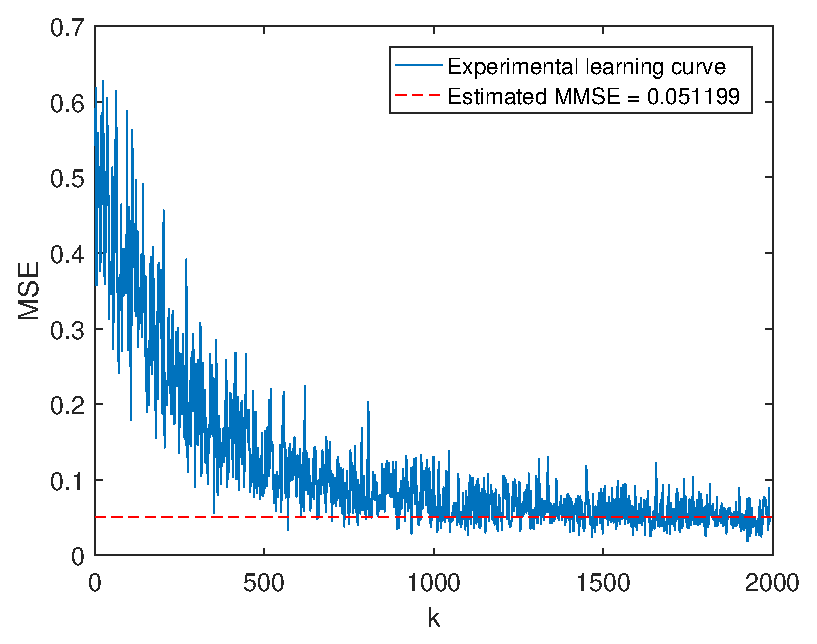
\includegraphics[scale=0.8]{figs/part1_learning_curve.eps}
			\caption{Experimental learning curve for nonlinear plant indemnification using a linear filter. The learning curve was averaged 100 times.}
			\label{fig:part1-learning-curve}
		\end{figure}
		\FloatBarrier
		
		\FloatBarrier
		\begin{figure}[h!]
			\centering
			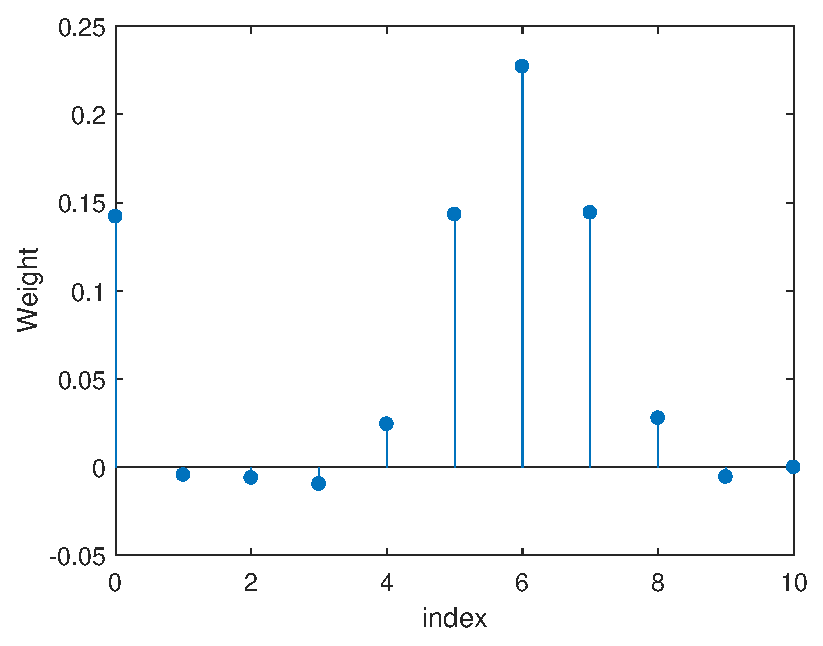
\includegraphics[scale=0.8]{figs/part1_weights.eps}
			\caption{Weight vector after convergence.}
			\label{fig:part1-weights}
		\end{figure}
		\FloatBarrier
	}
	\fi
	
	\item (5 points) Use the last 200 samples of the averaged learning curve to estimate the minimum mean square error (MMSE) and report its value. 
	
	\if\SOLUTIONS1 {\color{\SolutionsColor}
		As shown in Figure~\ref{fig:part1-learning-curve}, the MMSE estimated using the last 200 samples was equal to $\approx 0.051$.
	}
	\fi
		
	\item (5 points) Apply the test signal $x_{test}[n] = 2\cos\big(\frac{\pi}{10} n\big), n = 0, 1,\ldots, 50$ to the plant and to the converged adaptive filter and plot their outputs on the same graph. Explain any discrepancies. As in part (b), you should use the weights obtained at the last iteration of the last run. Note that you trained the adaptive filter with a random signal, and now you're testing it with a deterministic sinusoidal signal. 
	
	Note: During testing you should treat the adaptive filter as a fixed filter whose coefficients are the coefficients you plotted in part (b).
	
	\if\SOLUTIONS1 {\color{\SolutionsColor}
		The Matlab code is the same as for part (b) and it is shown below. The output of the plant is compared to the output of the adaptive filter in Figure~\ref{fig:part1-test}.
		
		\FloatBarrier
		\begin{figure}[h!]
			\centering
			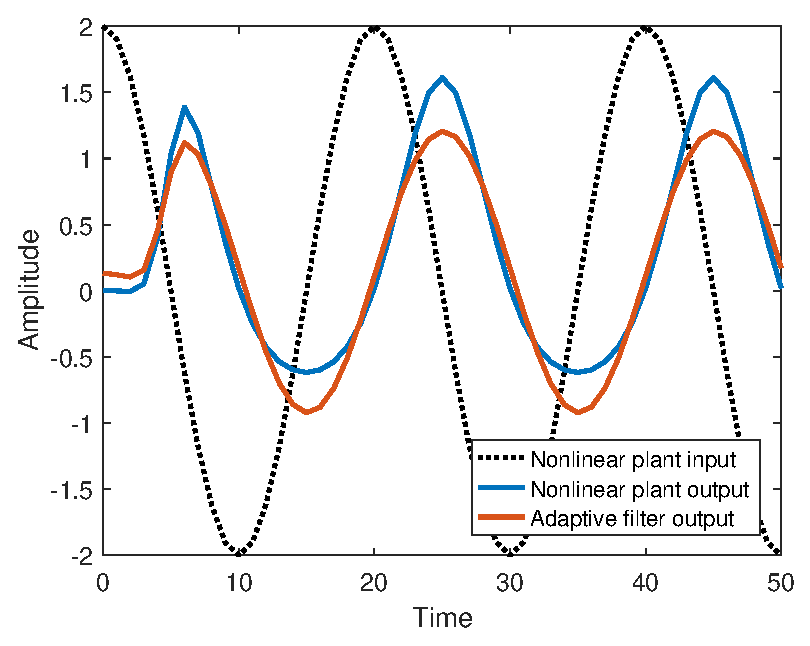
\includegraphics[scale=0.8]{figs/part1_test.eps}
			\caption{Test of the adaptive filter after convergence with a sinusoidal signal. During the first $L+1$ samples, the filter was being initialized.}
			\label{fig:part1-test}
		\end{figure}
		\FloatBarrier
	}
	\fi
	
	\if\SOLUTIONS1
	\textbf{Matlab code for part 1}
	% This file was automatically created from the m-file 
% "m2tex.m" written by USL. 
% The fontencoding in this file is UTF-8. 
%  
% You will need to include the following two packages in 
% your LaTeX-Main-File. 
%  
% \usepackage{color} 
% \usepackage{fancyvrb} 
%  
% It is advised to use the following option for Inputenc 
% \usepackage[utf8]{inputenc} 
%  
  
% definition of matlab colors: 
\definecolor{mblue}{rgb}{0,0,1} 
\definecolor{mgreen}{rgb}{0.13333,0.5451,0.13333} 
\definecolor{mred}{rgb}{0.62745,0.12549,0.94118} 
\definecolor{mgrey}{rgb}{0.5,0.5,0.5} 
\definecolor{mdarkgrey}{rgb}{0.25,0.25,0.25} 
  
\DefineShortVerb[fontfamily=courier,fontseries=m]{\$} 
\DefineShortVerb[fontfamily=courier,fontseries=b]{\#} 
  
\noindent                                                                         
 \hspace*{-1.6em}{\scriptsize 1}$  $\color{mgrey}#%% Part 1: Modeling nonlinear plant with linear adaptive filter#\color{black}$$\\
 \hspace*{-1.6em}{\scriptsize 2}$  Niterations = 2000;             $\color{mgrey}$% Number of iterations$\color{black}$$\\
 \hspace*{-1.6em}{\scriptsize 3}$  Nruns = 100;                    $\color{mgrey}$% Number of runs to average MSE$\color{black}$$\\
 \hspace*{-1.6em}{\scriptsize 4}$  L = 9;                          $\color{mgrey}$% Memory length$\color{black}$$\\
 \hspace*{-1.6em}{\scriptsize 5}$  var_r = 4;                      $\color{mgrey}$% variance of input signal$\color{black}$$\\
 \hspace*{-1.6em}{\scriptsize 6}$  xtest = 2*cos(pi/10*(0:50));    $\color{mgrey}$% test signal$\color{black}$$\\
 \hspace*{-1.6em}{\scriptsize 7}$  ytest = nonlinear_plant(xtest); $\color{mgrey}$% nonlinear plant output for test signal$\color{black}$$\\
 \hspace*{-1.6em}{\scriptsize 8}$  Nweights = L + 2;               $\color{mgrey}$% number of weights: FIR taps + bias weight$\color{black}$$\\
 \hspace*{-1.6em}{\scriptsize 9}$  $\\
 \hspace*{-2em}{\scriptsize 10}$  $\color{mgrey}$% Calculate mu$\color{black}$$\\
 \hspace*{-2em}{\scriptsize 11}$  mu_max = 1/(var_r*(L+1) + 1);   $\color{mgrey}$% mu_max = 1/tr(R)$\color{black}$$\\
 \hspace*{-2em}{\scriptsize 12}$  mu = 0.01*mu_max;               $\color{mgrey}$% adaptation constant$\color{black}$$\\
 \hspace*{-2em}{\scriptsize 13}$  $\\
 \hspace*{-2em}{\scriptsize 14}$  $\color{mgrey}$% Adaptation using LMS$\color{black}$$\\
 \hspace*{-2em}{\scriptsize 15}$  MSE = zeros(Niterations, Nruns);$\\
 \hspace*{-2em}{\scriptsize 16}$  $#for#$ run = 1:Nruns$\\
 \hspace*{-2em}{\scriptsize 17}$      $\color{mgrey}$% Input signal: white and uniformly distributed zero-mean noise with$\color{black}$$\\
 \hspace*{-2em}{\scriptsize 18}$      $\color{mgrey}$% var_r variance$\color{black}$$\\
 \hspace*{-2em}{\scriptsize 19}$      r = sqrt(var_r*12)*(rand(Niterations, 1)-0.5);$\\
 \hspace*{-2em}{\scriptsize 20}$  $\\
 \hspace*{-2em}{\scriptsize 21}$      d = nonlinear_plant(r); $\color{mgrey}$% calculate desired response$\color{black}$$\\
 \hspace*{-2em}{\scriptsize 22}$      $\\
 \hspace*{-2em}{\scriptsize 23}$      $\color{mgrey}$% Reset weights, input, and error before running LMS$\color{black}$$\\
 \hspace*{-2em}{\scriptsize 24}$      W = zeros(Nweights, 1); $\color{mgrey}$% weight vector$\color{black}$$\\
 \hspace*{-2em}{\scriptsize 25}$      X = zeros(L+1, 1); $\color{mgrey}$% shift register$\color{black}$$\\
 \hspace*{-2em}{\scriptsize 26}$      error = zeros(Niterations, 1);$\\
 \hspace*{-2em}{\scriptsize 27}$      $#for#$ k = 1:Niterations$\\
 \hspace*{-2em}{\scriptsize 28}$          X = [r(k); X(1:end-1)];     $\color{mgrey}$% tap delay line$\color{black}$$\\
 \hspace*{-2em}{\scriptsize 29}$          Xin = [1; X];               $\color{mgrey}$% append input for bias weigth W(1)$\color{black}$$\\
 \hspace*{-2em}{\scriptsize 30}$          y = W.'*Xin;                $\color{mgrey}$% calculate output$\color{black}$$\\
 \hspace*{-2em}{\scriptsize 31}$          error(k) = d(k) - y;        $\color{mgrey}$% calculate error$\color{black}$$\\
 \hspace*{-2em}{\scriptsize 32}$          W = W + 2*mu*error(k)*Xin;  $\color{mgrey}$% weight update$\color{black}$$\\
 \hspace*{-2em}{\scriptsize 33}$      $#end#$$\\
 \hspace*{-2em}{\scriptsize 34}$      MSE(:, $\color{mdarkgrey}$run) = error.^2;$\color{black}$$\\
 \hspace*{-2em}{\scriptsize 35}$  $#end#$$\\
 \hspace*{-2em}{\scriptsize 36}$  $\\
 \hspace*{-2em}{\scriptsize 37}$  MSE = mean(MSE, 2); $\color{mgrey}$% average MSE over the number of runs$\color{black}$$\\
 \hspace*{-2em}{\scriptsize 38}$  MMSE = mean(MSE(end-199:end)); $\color{mgrey}$% use last 200 samples to estimate MMSE$\color{black}$$\\
 \hspace*{-2em}{\scriptsize 39}$  $\\
 \hspace*{-2em}{\scriptsize 40}$  $\color{mgrey}$% Ouput for test signal using linear model. W(1) is the bias weight$\color{black}$$\\
 \hspace*{-2em}{\scriptsize 41}$  ymodel = filter(W(2:end), 1, xtest) + W(1);$\\
 \hspace*{-2em}{\scriptsize 42}$  $\\
 \hspace*{-2em}{\scriptsize 43}$  $\color{mgrey}#%% Plots#\color{black}$$\\
 \hspace*{-2em}{\scriptsize 44}$  $\color{mgrey}$% Learning curve$\color{black}$$\\
 \hspace*{-2em}{\scriptsize 45}$  figure, $\color{mdarkgrey}$hold on, box on$\color{black}$$\\
 \hspace*{-2em}{\scriptsize 46}$  plot(MSE(L+1:end))$\\
 \hspace*{-2em}{\scriptsize 47}$  plot([1 Niterations], MMSE*[1 1], $\color{mdarkgrey}$'--r'$\color{black}$)$\\
 \hspace*{-2em}{\scriptsize 48}$  xlabel($\color{mdarkgrey}$'k'$\color{black}$, $\color{mdarkgrey}$'Fontsize'$\color{black}$, 12)$\\
 \hspace*{-2em}{\scriptsize 49}$  ylabel($\color{mdarkgrey}$'MSE'$\color{black}$, $\color{mdarkgrey}$'Fontsize'$\color{black}$, 12)$\\
 \hspace*{-2em}{\scriptsize 50}$  set(gca, $\color{mdarkgrey}$'Fontsize'$\color{black}$, 12)$\\
 \hspace*{-2em}{\scriptsize 51}$  legend($\color{mdarkgrey}$'Experimental learning curve'$\color{black}$, sprintf($\color{mdarkgrey}$'Estimated MMSE = %G'$\color{black}$, MMSE))$\\
 \hspace*{-2em}{\scriptsize 52}$  saveas(gca, $\color{mdarkgrey}$'figs/part1_learning_curve'$\color{black}$, $\color{mdarkgrey}$'epsc'$\color{black}$)$\\
 \hspace*{-2em}{\scriptsize 53}$  $\\
 \hspace*{-2em}{\scriptsize 54}$  $\color{mgrey}$% Weights$\color{black}$$\\
 \hspace*{-2em}{\scriptsize 55}$  figure, $\color{mdarkgrey}$hold on, box on$\color{black}$$\\
 \hspace*{-2em}{\scriptsize 56}$  stem(0:length(W)-1, W, $\color{mdarkgrey}$'fill'$\color{black}$)$\\
 \hspace*{-2em}{\scriptsize 57}$  xlabel($\color{mdarkgrey}$'index'$\color{black}$, $\color{mdarkgrey}$'Fontsize'$\color{black}$, 12)$\\
 \hspace*{-2em}{\scriptsize 58}$  ylabel($\color{mdarkgrey}$'Weight'$\color{black}$, $\color{mdarkgrey}$'Fontsize'$\color{black}$, 12)$\\
 \hspace*{-2em}{\scriptsize 59}$  set(gca, $\color{mdarkgrey}$'Fontsize'$\color{black}$, 12)$\\
 \hspace*{-2em}{\scriptsize 60}$  saveas(gca, $\color{mdarkgrey}$'figs/part1_weights'$\color{black}$, $\color{mdarkgrey}$'epsc'$\color{black}$)$\\
 \hspace*{-2em}{\scriptsize 61}$  $\\
 \hspace*{-2em}{\scriptsize 62}$  $\color{mgrey}$% Test signal$\color{black}$$\\
 \hspace*{-2em}{\scriptsize 63}$  figure, $\color{mdarkgrey}$hold on, box on$\color{black}$$\\
 \hspace*{-2em}{\scriptsize 64}$  t = 0:50;$\\
 \hspace*{-2em}{\scriptsize 65}$  plot(t, xtest, $\color{mdarkgrey}$':k'$\color{black}$, $\color{mdarkgrey}$'LineWidth'$\color{black}$, 2)$\\
 \hspace*{-2em}{\scriptsize 66}$  plot(t, ytest, $\color{mdarkgrey}$'LineWidth'$\color{black}$, 2)$\\
 \hspace*{-2em}{\scriptsize 67}$  plot(t, ymodel, $\color{mdarkgrey}$'LineWidth'$\color{black}$, 2)$\\
 \hspace*{-2em}{\scriptsize 68}$  xlabel($\color{mdarkgrey}$'Time'$\color{black}$, $\color{mdarkgrey}$'FontSize'$\color{black}$, 12)$\\
 \hspace*{-2em}{\scriptsize 69}$  ylabel($\color{mdarkgrey}$'Amplitude'$\color{black}$, $\color{mdarkgrey}$'FontSize'$\color{black}$, 12)$\\
 \hspace*{-2em}{\scriptsize 70}$  set(gca, $\color{mdarkgrey}$'Fontsize'$\color{black}$, 12)$\\
 \hspace*{-2em}{\scriptsize 71}$  legend($\color{mdarkgrey}$'Nonlinear plant input'$\color{black}$, $\color{mdarkgrey}$'Nonlinear plant output'$\color{black}$,...$\\
 \hspace*{-2em}{\scriptsize 72}$      $\color{mdarkgrey}$'Adaptive filter output'$\color{black}$, $\color{mdarkgrey}$'Location'$\color{black}$, $\color{mdarkgrey}$'SouthEast'$\color{black}$)$\\
 \hspace*{-2em}{\scriptsize 73}$  saveas(gca, $\color{mdarkgrey}$'figs/part1_test'$\color{black}$, $\color{mdarkgrey}$'epsc'$\color{black}$)$\\ 
  
\UndefineShortVerb{\$} 
\UndefineShortVerb{\#}
	\fi
	
\end{enumerate}

\subsection*{Part II. Nonlinear adaptive filter}

Now let's model the plant using the nonlinear adaptive filter based on the truncated Volterra series. Similarly to part I, assume that $L = 9$, but now we have a total of $2(L+1) + \binom{L+1}{2} + 1 = 66$ weights.

\begin{enumerate}[label=(\alph*)]
	\item (10 points) Describe how we can use the LMS algorithm to adapt the weights. Specifically, what should be the input vector $X_n$ and the weight vector $W$ in the LMS weight update equation? Your answers should be in terms of the input signal $r[n], \ldots, r_[n-L]$, and the weights $w_0, w_1(l), w_2(l), l = 0, \ldots, L$, and $w_1(l_1, l_2), l_1\neq l_2$.  
	
	\if\SOLUTIONS1 {\color{\SolutionsColor}
		The input vector $X_n$ and the weight vector $W$ must be such that their inner product $X_n^TW$ is equivalent to \eqref{eq:volterra}. By inspection, 
		
		\begin{equation}
		X_n = \begin{bmatrix}
		1 \\
		r[n] \\
		r[n-1] \\
		\vdots \\
		r[n-L] \\
		r[n]^2 \\
		r[n-1]^2 \\
		\vdots \\
		r[n-L]^2 \\
		r[n]r[n-1] \\
		r[n]r[n-2] \\
		\vdots \\
		r[n-L+1]r[n-L]
		\end{bmatrix} \qquad W = \begin{bmatrix}
		w_0 \\
		w_2(0) \\
		w_2(1) \\
		\vdots \\
		w_2(L) \\
		w_1(0) \\
		w_1(1) \\
		\vdots \\
		w_1(L) \\
		w_1(0, 1) \\
		w_1(0, 2) \\
		\vdots \\
		w_1(L-1, L)
		\end{bmatrix}.
		\end{equation}
		
		This way the output of the linear combiner $X_n^TW$ is equal to \eqref{eq:volterra}. And we can use the LMS update equations as usual
		\begin{align}
		W \leftarrow W + 2\mu e[n]X_n \\
		\epsilon[n] = d[n] - X_n^TW
		\end{align}
	}
	\fi
	
	\item (10 points) Implement your method from part (a) and train the adaptive filter using a white and uniformly distributed input signal $r[n]$ with zero mean and variance $\sigma_r^2 = 4$. Assume $\mu = 4\times 10^{-4}$ and adapt over 2000 iterations. Plot the learning curve averaged over 100 independent input realizations. On a separate graph, plot the converged weight vector obtained at the last iteration of the last  run. 
	
	\if\SOLUTIONS1 {\color{\SolutionsColor}
		The Matlab code to calculate the learning curve is included below. Figure~\ref{fig:part2-learning-curve} shows the learning curve averaged over 100 independent input realizations, and  Figure~\ref{fig:part2-weights} shows the converged weight vector. 
		
		Note that the learning curve converged to a much smaller MMSE. Note further that the bias weight is practically negligible now, and some of the weights corresponding to the squared inputs and to the cross-products are significant. 
		
		\FloatBarrier
		\begin{figure}[h!]
			\centering
			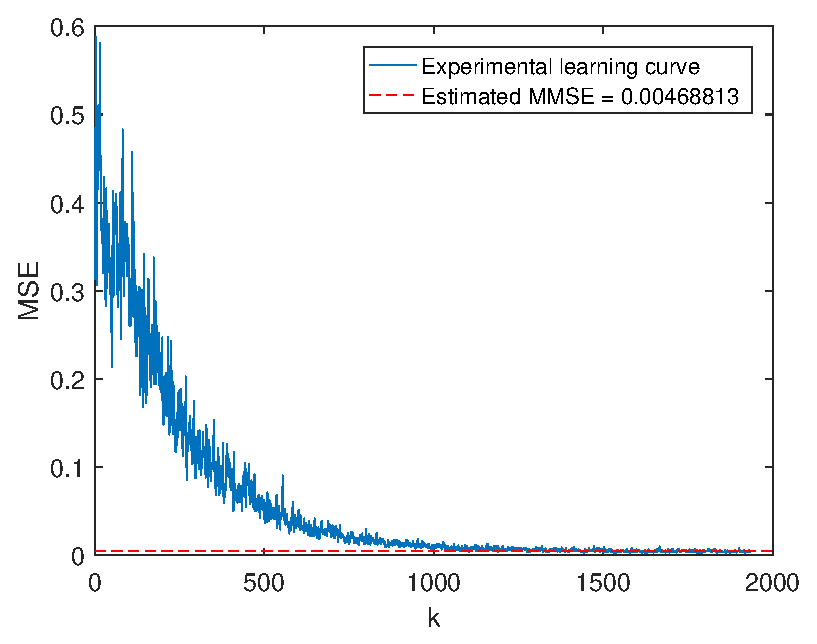
\includegraphics[scale=0.8]{figs/part2_learning_curve.eps}
			\caption{Experimental learning curve for nonlinear plant identification using a nonlinear filter based on Volterra series. The learning curve was averaged 100 times. The training signal had variance $\sigma_r^2 = 4$.}
			\label{fig:part2-learning-curve}
		\end{figure}
		\FloatBarrier
		
		\FloatBarrier
		\begin{figure}[h!]
			\centering
			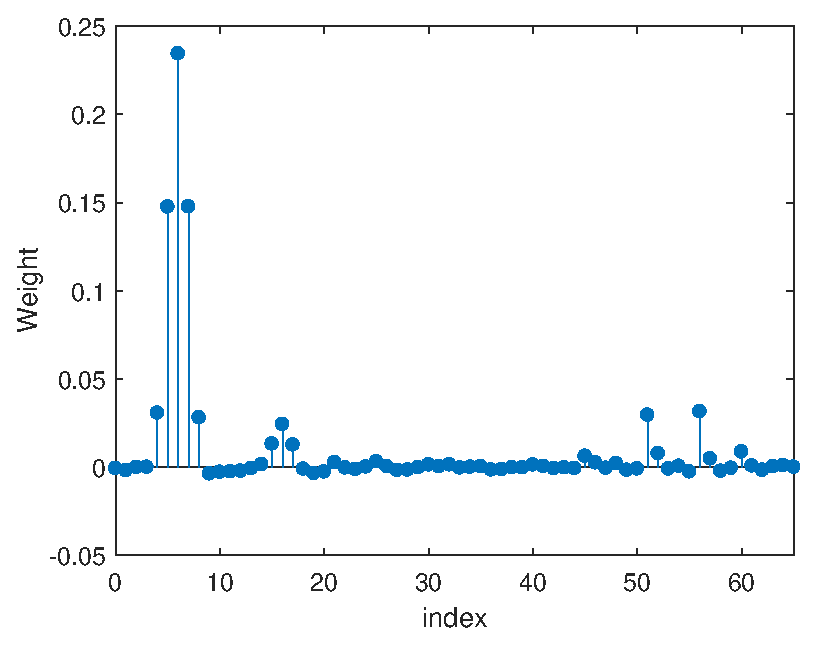
\includegraphics[scale=0.8]{figs/part2_weights.eps}
			\caption{Weight vector after convergence.}
			\label{fig:part2-weights}
		\end{figure}
		\FloatBarrier
	}
	\fi
	
	\item (5 points) Use the last 200 samples of the averaged learning curve to estimate the MMSE. Compare this result to what you obtained in Part I(c). 
	
	\if\SOLUTIONS1 {\color{\SolutionsColor}
		As shown in Figure~\ref{fig:part2-learning-curve}, the MMSE estimated using the last 200 samples was equal to $\approx 0.0046$.
	}
	\fi
	
	\item (5 points) Apply the test signal $x_{test}[n] = 2\cos\big(\frac{\pi}{10} n\big), n = 0, 1,\ldots, 50$ to the plant and to the converged adaptive filter and plot their outputs on the same graph. As before, use the weights obtained at the last iteration of the last run. Was there any improvement compared to Part 1(e)? 
	
	\if\SOLUTIONS1 {\color{\SolutionsColor}
	The Matlab code is included in the appendix. The output of the plant is compared to the output of the adaptive filter in Figure~\ref{fig:part2-test}. 
	
	The adaptive filter was trained with random signal, but it can almost perfectly track the plant output to a sinusoidal input. The same cannot be accomplished when the adaptive filter is linear as in part 1.E.

		\FloatBarrier
		\begin{figure}[h!]
			\centering
			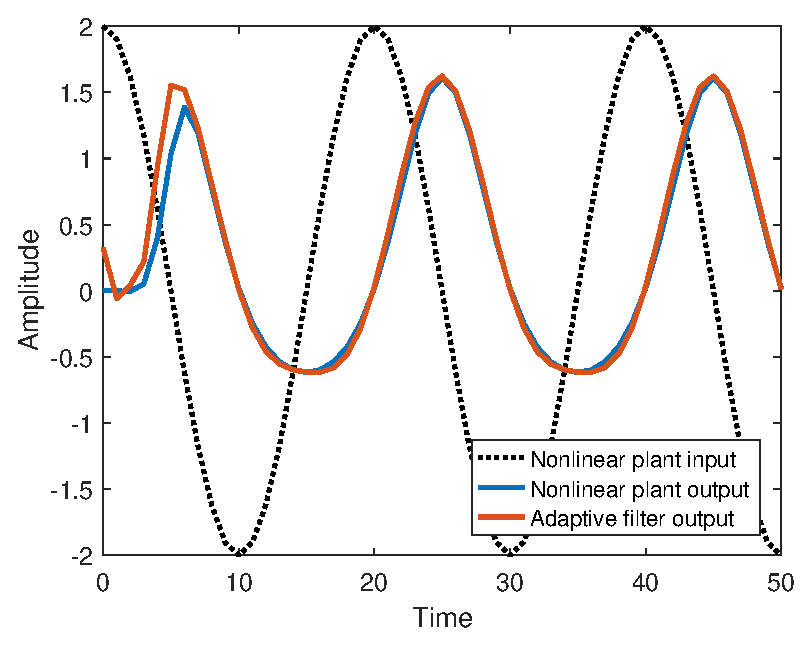
\includegraphics[scale=0.8]{figs/part2_test.eps}
			\caption{Test of the adaptive filter after convergence with a sinusoidal signal. During the first $L+1$ samples, the filter was being initialized.}
			\label{fig:part2-test}
		\end{figure}
		\FloatBarrier
	}
	\fi
	
\end{enumerate}

\if\SOLUTIONS1
\textbf{Matlab code for part 2}
% This file was automatically created from the m-file 
% "m2tex.m" written by USL. 
% The fontencoding in this file is UTF-8. 
%  
% You will need to include the following two packages in 
% your LaTeX-Main-File. 
%  
% \usepackage{color} 
% \usepackage{fancyvrb} 
%  
% It is advised to use the following option for Inputenc 
% \usepackage[utf8]{inputenc} 
%  
  
% definition of matlab colors: 
\definecolor{mblue}{rgb}{0,0,1} 
\definecolor{mgreen}{rgb}{0.13333,0.5451,0.13333} 
\definecolor{mred}{rgb}{0.62745,0.12549,0.94118} 
\definecolor{mgrey}{rgb}{0.5,0.5,0.5} 
\definecolor{mdarkgrey}{rgb}{0.25,0.25,0.25} 
  
\DefineShortVerb[fontfamily=courier,fontseries=m]{\$} 
\DefineShortVerb[fontfamily=courier,fontseries=b]{\#} 
  
\noindent                                                                                      
 \hspace*{-1.6em}{\scriptsize 1}$  $\color{mgrey}#%% Part 2: Modeling nonlinear plant with nonlinear adaptive filter#\color{black}$$\\
 \hspace*{-1.6em}{\scriptsize 2}$  Niterations = 2000;             $\color{mgrey}$% Number of iterations$\color{black}$$\\
 \hspace*{-1.6em}{\scriptsize 3}$  Nruns = 100;                    $\color{mgrey}$% Number of runs to average MSE$\color{black}$$\\
 \hspace*{-1.6em}{\scriptsize 4}$  L = 9;                          $\color{mgrey}$% filter length - 1$\color{black}$$\\
 \hspace*{-1.6em}{\scriptsize 5}$  var_r = 4;                      $\color{mgrey}$% variance of input signal$\color{black}$$\\
 \hspace*{-1.6em}{\scriptsize 6}$  mu = 4e-4;                      $\color{mgrey}$% adaptation constant$\color{black}$$\\
 \hspace*{-1.6em}{\scriptsize 7}$  xtest = 2*cos(pi/10*(0:50));    $\color{mgrey}$% test signal$\color{black}$$\\
 \hspace*{-1.6em}{\scriptsize 8}$  ytest = nonlinear_plant(xtest); $\color{mgrey}$% nonlinear plant output for test signal$\color{black}$$\\
 \hspace*{-1.6em}{\scriptsize 9}$  Nweights = 2*(L+1) + nchoosek(L+1, 2) + 1; $\color{mgrey}$% Number of weights$\color{black}$$\\
 \hspace*{-2em}{\scriptsize 10}$  $\\
 \hspace*{-2em}{\scriptsize 11}$  $\color{mgrey}$% For part 2.E$\color{black}$$\\
 \hspace*{-2em}{\scriptsize 12}$  $\color{mgrey}$% var_r = 0.4;$\color{black}$$\\
 \hspace*{-2em}{\scriptsize 13}$  $\color{mgrey}$% mu = 4e-3;$\color{black}$$\\
 \hspace*{-2em}{\scriptsize 14}$  $\\
 \hspace*{-2em}{\scriptsize 15}$  $\color{mgrey}$% Indices for cross-products $\color{black}$$\\
 \hspace*{-2em}{\scriptsize 16}$  idx = nchoosek(1:L+1, 2);       $\\
 \hspace*{-2em}{\scriptsize 17}$  $\\
 \hspace*{-2em}{\scriptsize 18}$  MSE = zeros(Niterations, Nruns);$\\
 \hspace*{-2em}{\scriptsize 19}$  $#for#$ run = 1:Nruns$\\
 \hspace*{-2em}{\scriptsize 20}$      $\color{mgrey}$% Input signal: white and uniformly distributed zero-mean noise with$\color{black}$$\\
 \hspace*{-2em}{\scriptsize 21}$      $\color{mgrey}$% var_r variance$\color{black}$$\\
 \hspace*{-2em}{\scriptsize 22}$      r = sqrt(var_r*12)*(rand(Niterations, 1)-0.5); $\\
 \hspace*{-2em}{\scriptsize 23}$  $\\
 \hspace*{-2em}{\scriptsize 24}$      d = nonlinear_plant(r); $\color{mgrey}$% calculate desired response$\color{black}$$\\
 \hspace*{-2em}{\scriptsize 25}$      $\\
 \hspace*{-2em}{\scriptsize 26}$      $\color{mgrey}$% Reset weights, input, and error before running LMS$\color{black}$$\\
 \hspace*{-2em}{\scriptsize 27}$      W = zeros(Nweights, 1); $\color{mgrey}$% weight vector$\color{black}$$\\
 \hspace*{-2em}{\scriptsize 28}$      X = zeros(L+1, 1); $\color{mgrey}$% shift register$\color{black}$$\\
 \hspace*{-2em}{\scriptsize 29}$      error = zeros(Niterations, 1);$\\
 \hspace*{-2em}{\scriptsize 30}$      $#for#$ k = 1:Niterations$\\
 \hspace*{-2em}{\scriptsize 31}$          X = [r(k); X(1:end-1)];                 $\color{mgrey}$% tap delay line$\color{black}$$\\
 \hspace*{-2em}{\scriptsize 32}$          X2 = X.^2;                              $\color{mgrey}$% squared inputs $\color{black}$$\\
 \hspace*{-2em}{\scriptsize 33}$          Xprod  = X(idx(:, 1)).*X(idx(:, 2));    $\color{mgrey}$% cross-products$\color{black}$$\\
 \hspace*{-2em}{\scriptsize 34}$          Xin = [1; X; X2; Xprod];                $\color{mgrey}$% build input to adaptive filter$\color{black}$$\\
 \hspace*{-2em}{\scriptsize 35}$          y = W.'*Xin;                            $\color{mgrey}$% calculate output$\color{black}$$\\
 \hspace*{-2em}{\scriptsize 36}$          error(k) = d(k) - y;                    $\color{mgrey}$% calculate error$\color{black}$$\\
 \hspace*{-2em}{\scriptsize 37}$          W = W + 2*mu*error(k)*Xin;              $\color{mgrey}$% weights update$\color{black}$$\\
 \hspace*{-2em}{\scriptsize 38}$      $#end#$$\\
 \hspace*{-2em}{\scriptsize 39}$      MSE(:, $\color{mdarkgrey}$run) = error.^2;$\color{black}$$\\
 \hspace*{-2em}{\scriptsize 40}$  $#end#$$\\
 \hspace*{-2em}{\scriptsize 41}$  $\\
 \hspace*{-2em}{\scriptsize 42}$  MSE = mean(MSE, 2); $\color{mgrey}$% average MSE over the number of runs$\color{black}$$\\
 \hspace*{-2em}{\scriptsize 43}$  MMSE = mean(MSE(end-199:end)); $\color{mgrey}$% use last 200 samples to estimate MMSE$\color{black}$$\\
 \hspace*{-2em}{\scriptsize 44}$  $\\
 \hspace*{-2em}{\scriptsize 45}$  $\color{mgrey}$% Calculate model output for test signal$\color{black}$$\\
 \hspace*{-2em}{\scriptsize 46}$  ymodel = zeros(size(xtest));$\\
 \hspace*{-2em}{\scriptsize 47}$  $#for#$ k = 1:length(xtest)$\\
 \hspace*{-2em}{\scriptsize 48}$      X = [xtest(k); X(1:end-1)];$\\
 \hspace*{-2em}{\scriptsize 49}$      X2 = X.^2;$\\
 \hspace*{-2em}{\scriptsize 50}$      Xprod  = X(idx(:, 1)).*X(idx(:, 2));$\\
 \hspace*{-2em}{\scriptsize 51}$      Xin = [1; X; X2; Xprod];$\\
 \hspace*{-2em}{\scriptsize 52}$      ymodel(k) = W.'*Xin;$\\
 \hspace*{-2em}{\scriptsize 53}$  $#end#$$\\
 \hspace*{-2em}{\scriptsize 54}$  $\\
 \hspace*{-2em}{\scriptsize 55}$  $\color{mgrey}#%% Plots#\color{black}$$\\
 \hspace*{-2em}{\scriptsize 56}$  $\color{mgrey}$% Learning curve$\color{black}$$\\
 \hspace*{-2em}{\scriptsize 57}$  figure, $\color{mdarkgrey}$hold on, box on$\color{black}$$\\
 \hspace*{-2em}{\scriptsize 58}$  plot(MSE(Nweights+1:end, $\color{mdarkgrey}$:))$\color{black}$$\\
 \hspace*{-2em}{\scriptsize 59}$  plot([1 Niterations], MMSE*[1 1], $\color{mdarkgrey}$'--r'$\color{black}$)$\\
 \hspace*{-2em}{\scriptsize 60}$  xlabel($\color{mdarkgrey}$'k'$\color{black}$, $\color{mdarkgrey}$'Fontsize'$\color{black}$, 12)$\\
 \hspace*{-2em}{\scriptsize 61}$  ylabel($\color{mdarkgrey}$'MSE'$\color{black}$, $\color{mdarkgrey}$'Fontsize'$\color{black}$, 12)$\\
 \hspace*{-2em}{\scriptsize 62}$  set(gca, $\color{mdarkgrey}$'Fontsize'$\color{black}$, 12)$\\
 \hspace*{-2em}{\scriptsize 63}$  legend($\color{mdarkgrey}$'Experimental learning curve'$\color{black}$, sprintf($\color{mdarkgrey}$'Estimated MMSE = %G'$\color{black}$, MMSE))$\\
 \hspace*{-2em}{\scriptsize 64}$  saveas(gca, $\color{mdarkgrey}$'figs/part2_learning_curve'$\color{black}$, $\color{mdarkgrey}$'epsc'$\color{black}$)$\\
 \hspace*{-2em}{\scriptsize 65}$  $\\
 \hspace*{-2em}{\scriptsize 66}$  $\color{mgrey}$% Weights$\color{black}$$\\
 \hspace*{-2em}{\scriptsize 67}$  figure, $\color{mdarkgrey}$hold on, box on$\color{black}$$\\
 \hspace*{-2em}{\scriptsize 68}$  stem(0:Nweights-1, W, $\color{mdarkgrey}$'fill'$\color{black}$)$\\
 \hspace*{-2em}{\scriptsize 69}$  xlabel($\color{mdarkgrey}$'index'$\color{black}$, $\color{mdarkgrey}$'Fontsize'$\color{black}$, 12)$\\
 \hspace*{-2em}{\scriptsize 70}$  ylabel($\color{mdarkgrey}$'Weight'$\color{black}$, $\color{mdarkgrey}$'Fontsize'$\color{black}$, 12)$\\
 \hspace*{-2em}{\scriptsize 71}$  set(gca, $\color{mdarkgrey}$'Fontsize'$\color{black}$, 12)$\\
 \hspace*{-2em}{\scriptsize 72}$  axis([0 $\color{mdarkgrey}$Nweights-1 -0.05 0.25])$\color{black}$$\\
 \hspace*{-2em}{\scriptsize 73}$  saveas(gca, $\color{mdarkgrey}$'figs/part2_weights'$\color{black}$, $\color{mdarkgrey}$'epsc'$\color{black}$)$\\
 \hspace*{-2em}{\scriptsize 74}$  $\\
 \hspace*{-2em}{\scriptsize 75}$  $\color{mgrey}$% Test signal$\color{black}$$\\
 \hspace*{-2em}{\scriptsize 76}$  figure, $\color{mdarkgrey}$hold on, box on$\color{black}$$\\
 \hspace*{-2em}{\scriptsize 77}$  t = 0:50;$\\
 \hspace*{-2em}{\scriptsize 78}$  plot(t, xtest, $\color{mdarkgrey}$':k'$\color{black}$, $\color{mdarkgrey}$'LineWidth'$\color{black}$, 2)$\\
 \hspace*{-2em}{\scriptsize 79}$  plot(t, ytest, $\color{mdarkgrey}$'LineWidth'$\color{black}$, 2)$\\
 \hspace*{-2em}{\scriptsize 80}$  plot(t, ymodel, $\color{mdarkgrey}$'LineWidth'$\color{black}$, 2)$\\
 \hspace*{-2em}{\scriptsize 81}$  xlabel($\color{mdarkgrey}$'Time'$\color{black}$, $\color{mdarkgrey}$'FontSize'$\color{black}$, 12)$\\
 \hspace*{-2em}{\scriptsize 82}$  ylabel($\color{mdarkgrey}$'Amplitude'$\color{black}$, $\color{mdarkgrey}$'FontSize'$\color{black}$, 12)$\\
 \hspace*{-2em}{\scriptsize 83}$  legend($\color{mdarkgrey}$'Nonlinear plant input'$\color{black}$, $\color{mdarkgrey}$'Nonlinear plant output'$\color{black}$,...$\\
 \hspace*{-2em}{\scriptsize 84}$      $\color{mdarkgrey}$'Adaptive filter output'$\color{black}$, $\color{mdarkgrey}$'Location'$\color{black}$, $\color{mdarkgrey}$'SouthEast'$\color{black}$)$\\
 \hspace*{-2em}{\scriptsize 85}$  set(gca, $\color{mdarkgrey}$'Fontsize'$\color{black}$, 12)$\\
 \hspace*{-2em}{\scriptsize 86}$  saveas(gca, $\color{mdarkgrey}$'figs/part2_test'$\color{black}$, $\color{mdarkgrey}$'epsc'$\color{black}$)$\\ 
  
\UndefineShortVerb{\$} 
\UndefineShortVerb{\#}
\fi
	

\end{document}
